\documentclass{article}
\usepackage{graphicx} % Required for inserting images
\usepackage[margin=3cm]{geometry} % Adjust the margin as needed
\usepackage{tabularx}
\usepackage[table]{xcolor} % Pacchetto per colorare le celle
\usepackage[italian]{babel}
\usepackage{float}
\usepackage{hyperref}
\usepackage{caption}

% \newcommand{\code}[1]{\textbf{\textcolor{cyan}{#1}}}
\newcommand{\code}[1]{\texttt{#1}}

\title{GreenHouse \\ \vspace{0.5cm} {Software per la gestione di serre e piante}}
\author{Elion Karaboja \\ \and Lorenzo Cappellini}
\date{Maggio - Ottobre 2024} 

\begin{document}

\begin{titlepage}

\newcommand{\HRule}{\rule{\linewidth}{0.5mm}} % Defines a new command for the horizontal lines, change thickness here

%----------------------------------------------------------------------------------------
%	LOGO SECTION
%----------------------------------------------------------------------------------------
\center

\includegraphics[width=14cm]{resources/images/Icons/icon_unifilogo.png}\\[1cm] % Include a department/university logo - this will require the graphicx package
 
%----------------------------------------------------------------------------------------

\center % Center everything on the page

%----------------------------------------------------------------------------------------
%	HEADING SECTIONS
%----------------------------------------------------------------------------------------

\textsc{\LARGE Università degli Studi di Firenze}\\[0.5cm] % Major heading such as course name
\textsc{\Large Dipartimento di Ingegneria dell'Informazione}\\[0.5cm] % Minor heading such as course title

%----------------------------------------------------------------------------------------
%	TITLE SECTION
%----------------------------------------------------------------------------------------
\makeatletter
\HRule \\[1cm]
{ \huge \bfseries \@title}\\[0.7cm] % Title of your document
\HRule \\[1.5cm]
 
%----------------------------------------------------------------------------------------
%	AUTHOR SECTION
%----------------------------------------------------------------------------------------

\begin{minipage}{0.4\textwidth}
\begin{flushleft} \large
\emph{Autori:}\\
Elion Karaboja \newline Lorenzo Cappellini
\\[1.2em]
\emph{N° Matricola:}\\
7030984 \newline 7049027\\[1.2em]
\end{flushleft}
\end{minipage}
~
\begin{minipage}{0.4\textwidth}
\begin{flushright} \large
\emph{Corso principale:} \\
Ingegneria del Software  \\[1.2em]
\emph{Docente corso:} \\
Enrico Vicario
\end{flushright}
\end{minipage}\\[2cm]
\makeatother


\vfill % Fill the rest of the page with whitespace

\end{titlepage}

\tableofcontents

\newpage
\section{Introduzione}
Elaborato per il superamento dell’esame di Ingegneria del Software, appartenente al modulo Basi di Dati / Ingegneria del Software del corso di Laurea Triennale in Ingegneria Informatica dell’Università degli Studi di Firenze.
\\

\noindent Il progetto è stato sviluppato da Elion Karaboja e Lorenzo Cappellini (matricole 7030984 e 7049027) durante il periodo di Maggio - Settembre 2024 (a.a. 2023/2024).
\\

\noindent Il codice sorgente è disponibile su Github al seguente indirizzo:\\ 
\href{https://github.com/lcappellini/SWE_Greenhouse}{https://github.com/lcappellini/SWE\_Greenhouse}.

\subsection{Statement}
Il progetto modella un sistema di controllo e gestione di serre, e in particolare si occupa della cura e crescita delle piante in esse, al fine ultimo di venderle a clienti. 
I 3 spazi delle serre sono divisi in 4 settori in cui è presente un sistema di areazione, di illuminazione e controllo della temperatura, luce e umidità, e contengono 5 posizioni ciascuna nelle quali mettere le piante che saranno irrigate e monitorate. \\
La gestione delle piante è in gran parte automatizzata e possono essere monitorati sia i settori che le posizioni per ottenere un controllo \textit{real-time} da parte dell'Admin.\\ Ci sono operazioni che dovranno essere effettuate manualmente come la cura e il posizionamento delle piante nelle posizioni designate, che saranno eseguite da operatori. Tale sistema è adottato da un'azienda che permette ai clienti di acquistare e commissionare un certo numero di piante con consegna prevista entro un certo periodo.
\subsection{Struttura e pratiche utilizzate}
Il software è stato sviluppato in Java, mentre per la gestione e il salvataggio dei dati è stato connesso un database PostgreSQL ed è stata utilizzata la libreria JDBC (Java DataBase Connectivity).
\\

\noindent Per mantenere una separazione delle responsabilità, la struttura del progetto è stata divisa in tre parti principali: Business Logic, Domain Model e ORM. Questi tre packages si occupano in modo distinto della logica di business, della rappresentazione dei dati e dell’accesso ai dati (Figura \ref{fig:diagram_packagedependency}):
\begin{itemize}
    \item \textbf{Business Logic}: contiene le classi che implementano la logica di business del sistema.
    \item \textbf{Domain Model}: contiene le classi che rappresentano le entità del sistema.
    \item \textbf{ORM}: contiene le classi che implementano l’Object-Relational Mapping. In questo modo è possibile rendere i dati persistenti e recuperarli dal database.
\end{itemize}
Per utilizzare il software è stata creata un’interfaccia da riga di comando (CLI) che permette di interagire con il sistema in modo semplice e intuitivo.
\\

\noindent Gli Use Case Diagram e i Class Diagram seguono lo standard UML (Unified Modeling Language) e sono stati realizzati con il software StarUML. Infine, per la parte di testing è stato utilizzato JUnit.
\begin{figure}[H]
    \centering
    \fbox{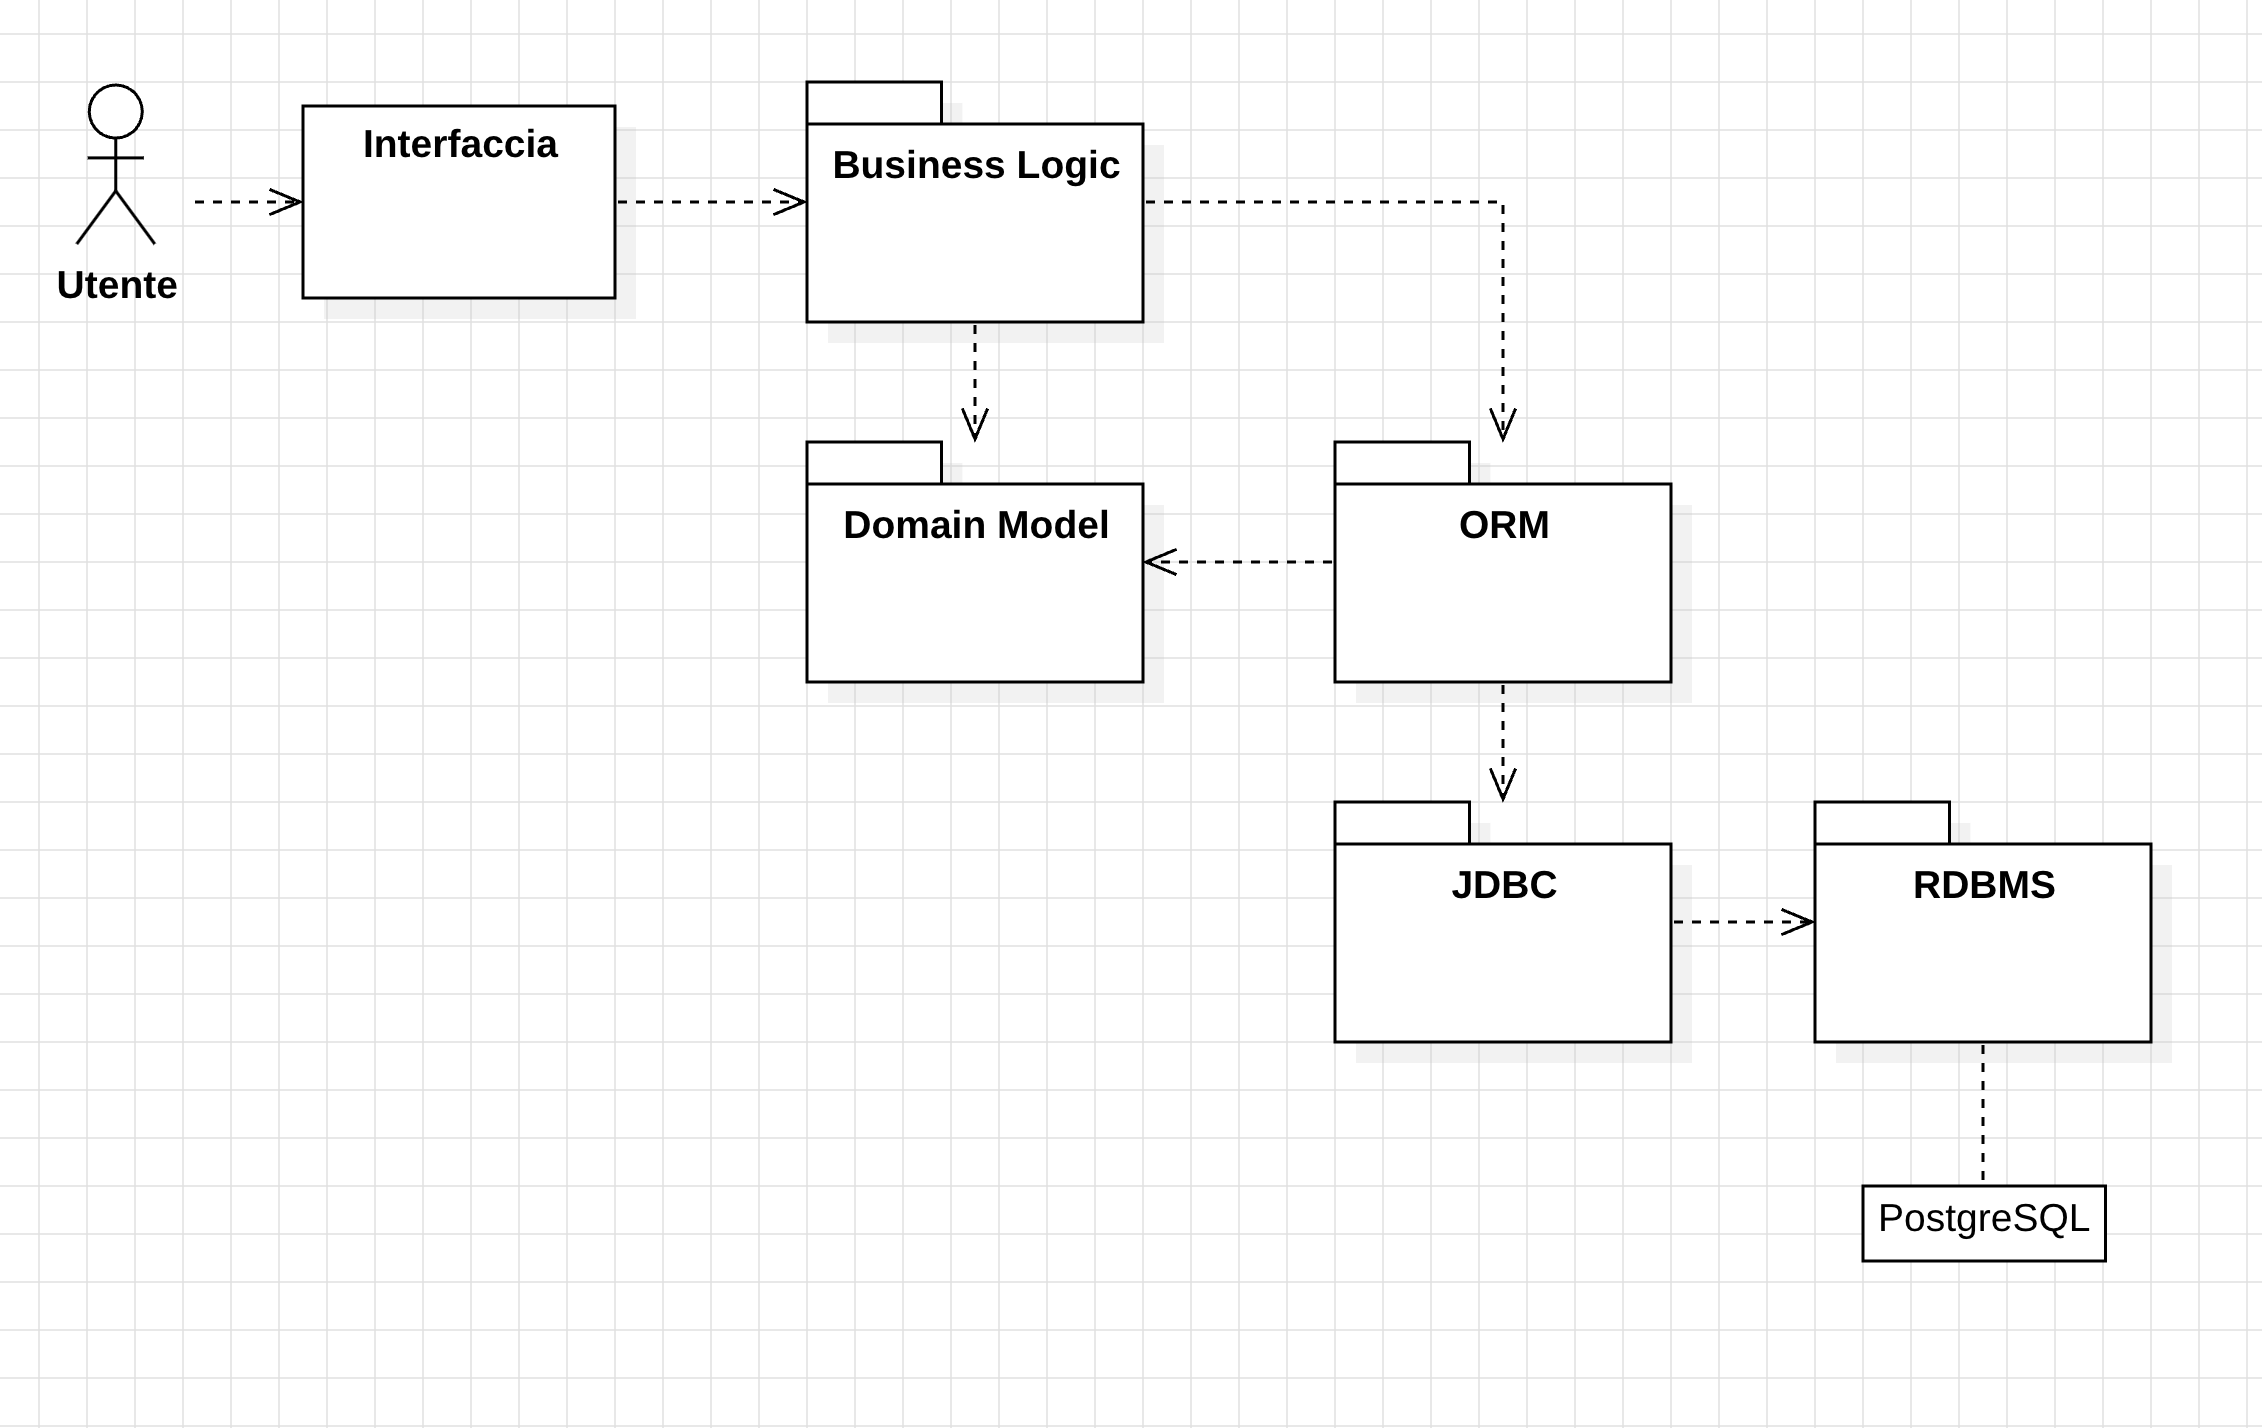
\includegraphics[scale=0.3]{resources/images/Diagrams/diagram_packagedependency.png}}
    \caption{Package Dependency Diagram}
    \label{fig:diagram_packagedependency}
\end{figure}

\newpage\section{Progettazione}

\subsection{Use Case Diagram}
Come descritto in precedenza, il sistema è stato progettato per permettere a clienti di ordinare e ritirare le piante desiderate, le quali sono gestite da operatori e monitorate da un Admin. La Figura \ref{fig:diagram_usecases} illustra il diagramma dei casi d'uso del sistema, includendo quelli relativi ai Clienti, agli Operatori e agli Admin.

\begin{figure}[H]
    \centering
    \fbox{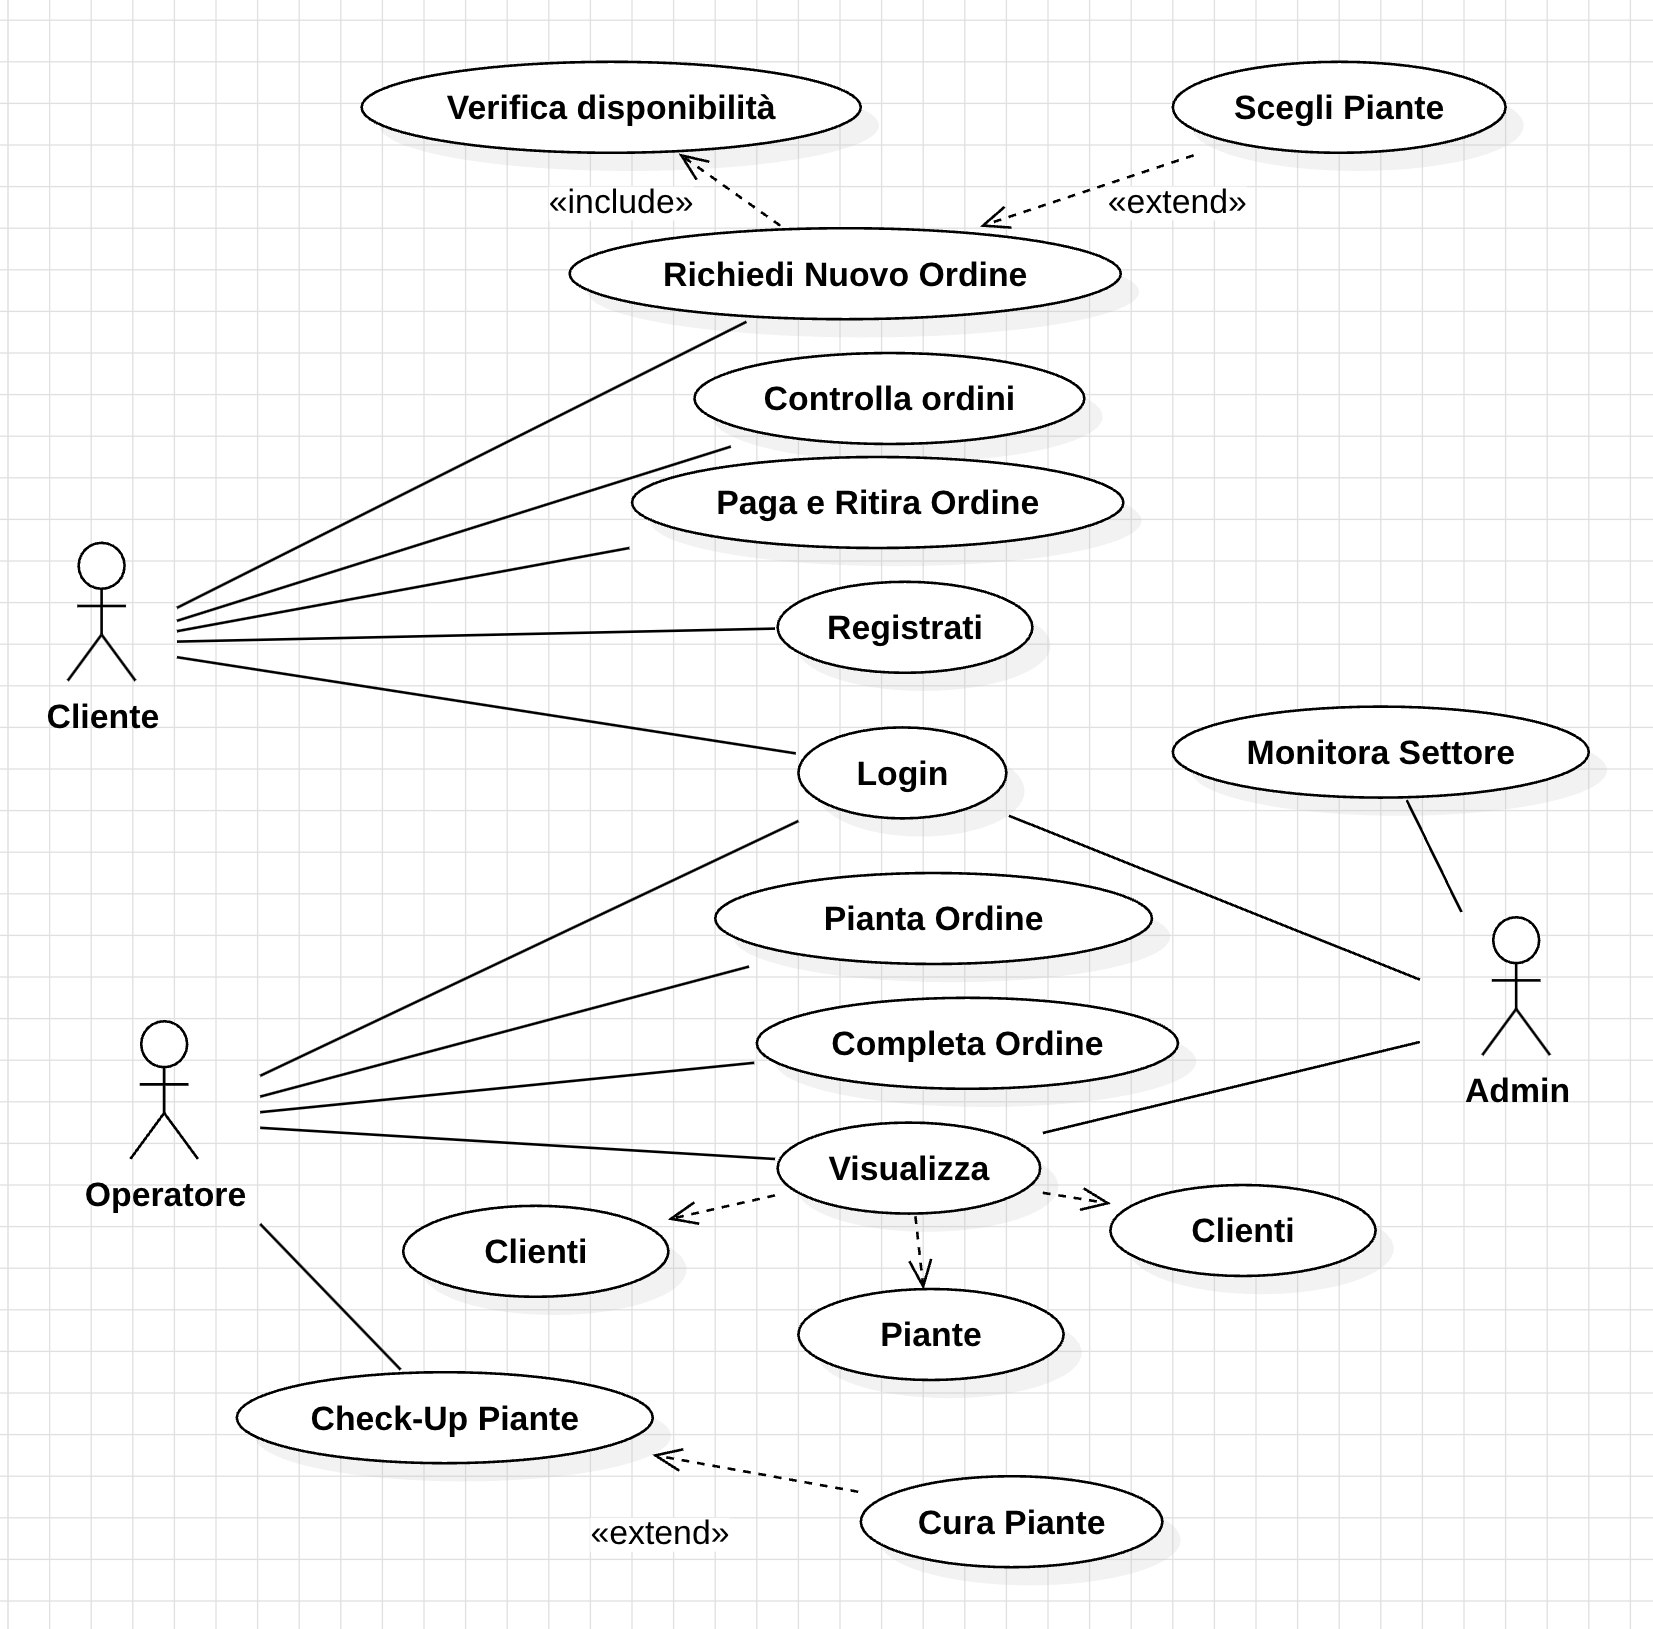
\includegraphics[scale=0.5]{resources/images/Diagrams/diagram_usecases.png}}
    \caption{Diagramma degli Use Cases}
    \label{fig:diagram_usecases}
\end{figure}

\subsection{Use Case Template}
Qui di seguito sono elencati i template di alcuni casi d'uso implementati. Per ciascuno sono specificati dei dettagli: una breve descrizione, il livello del caso d'uso, gli attori coinvolti, le precondizioni, le post-condizioni, il flusso principale e i flussi alternativi.

\renewcommand{\arraystretch}{1.5}

\begin{table}[p]
    \begin{tabularx}{\textwidth}{ | l  X | }
        \rowcolor{lightgray!70}
        \hline
        \textbf{Use Case \#1} & \textbf{Accedi al Sistema (Sign-in)}\\[0.5ex]
        \textbf{Brief Description} & L'utente accede al sistema tramite le proprie credenziali (\hyperref[fig:mockup_1]{Mockup \#1})\\
        \rowcolor{blue!10}
        \textbf{Level} & User Goal \\
        \textbf{Actors} & Admin, Cliente, Operatore \\
        \rowcolor{blue!10}
        \textbf{Pre-Conditions} & L'utente deve essere nella pagina dedicata al proprio accesso \\
        \textbf{Basic Flow} & 1) L'utente inserisce le proprie credenziali\\
        & 2) L'utente invia le proprie credenziali\\
        & 3) Il sistema verifica le credenziali\\
        & 4) Il sistema autentica l'utente \\        
        \rowcolor{blue!10}
        \textbf{Alternative Flow} & 3a) Se le credenziali sono errate, il sistema restituisce un messaggio di errore e permette di ritentare \\
        \textbf{Post-Conditions} & L'utente è autenticato nel sistema e ha accesso alle sue funzioni \\
        \hline
    \end{tabularx}
    \caption{Use Case \#1 (Accedi al Sistema)}
\end{table}


\begin{table}[p]
    \begin{tabularx}{\textwidth}{ | l  X | }
        \hline
        \rowcolor{lightgray!70}
        \textbf{Use Case \#2} & \textbf{Registrati nel Sistema (Sign-up)}\\ [0.5ex]
        \textbf{Brief Description} & Il cliente si registra nel sistema creando un nuovo account (\hyperref[fig:mockup_2]{Mockup \#2})\\
        \rowcolor{blue!10}
        \textbf{Level} & User Goal \\
        \textbf{Actors} & Cliente \\
        \rowcolor{blue!10}
        \textbf{Pre-Conditions} & Il cliente deve essere nella pagina di accesso del cliente\\
        \textbf{Basic Flow} & 1) Il cliente fornisce le informazioni richieste\\
        & 2) Il cliente conferma la registrazione\\
        & 3) Il sistema verifica i dati\\
        & 4) Il sistema crea un nuovo account per il cliente\\  
        \rowcolor{blue!10}
        \textbf{Alternative Flow} & 3a) Se il cliente fornisce dati non validi o già presenti (di un altro account), il sistema mostra un messaggio di errore\\
        \textbf{Post-Conditions} & Il cliente deve comunque effettuare il login per accedere al sistema\\
        \hline
    \end{tabularx}
    \caption{Use Case \#2 (Registrati  al Sistema)}
\end{table}


\begin{table}[p]
    \begin{tabularx}{\textwidth}{ | l  X | }
        \rowcolor{lightgray!70}
        \hline
        \textbf{Use Case \#3} & \textbf{Richiedi nuovo Ordine} \\[0.5ex]
        \textbf{Brief Description} & Il cliente crea un nuovo Ordine (\hyperref[fig:mockup_3]{Mockup \#3})\\
        \rowcolor{blue!10}
        \textbf{Level} & User Goal \\
        \textbf{Actors} & Cliente \\
        \rowcolor{blue!10}
        \textbf{Pre-Conditions} & Il cliente deve aver fatto l'accesso e essere nella pagina "Ordini" \\
        \textbf{Basic Flow} & 1) Il cliente seleziona l'opzione per creare un nuovo ordine\\
        & 2) Il cliente sceglie il tipo di pianta e la quantità desiderata\\
        & 3) Il cliente sceglie se aggiungere altre piante o se concludere l'ordine\\
        & 4) Il sistema registra il nuovo ordine\\
        \rowcolor{blue!10}
        \textbf{Alternative Flow} & 2a) Se il cliente inserisce valori non validi, il sistema mostra un messaggio di errore e richiede l'input\\
        \rowcolor{blue!10}
        & 4a) Se l'ordine non può essere preso in carico, il sistema restituisce un messaggio\\
        \textbf{Post-Conditions} & Il nuovo ordine è stato registrato nel sistema \\
        \hline
    \end{tabularx}
    \caption{Use Case \#3 (Richiedi nuovo Ordine)}
\end{table}


\begin{table}[p]
    \begin{tabularx}{\textwidth}{ | l  X | }
        \rowcolor{lightgray!70}
        \hline
        \textbf{Use Case \#4} & \textbf{Paga e Ritira Ordine }\\[0.5ex]
        \textbf{Brief Description} & Il cliente paga e ritira il proprio Ordine\\
        \rowcolor{blue!10}
        \textbf{Level} & User Goal \\
        \textbf{Actors} & Cliente \\
        \rowcolor{blue!10}
        \textbf{Pre-Conditions} & Il cliente è autenticato ed è nella sua pagina "Ordini" \\
        \textbf{Basic Flow} & 1) Il cliente seleziona l'opzione per pagare e ritirare l'ordine\\
        & 2) Il sistema mostra una lista di ordini pronti per essere ritirati\\
        & 3) Il cliente inserisce l'id dell'ordine scelto\\
        & 4) Il sistema conferma il pagamento e il ritiro di tale ordine\\
        \rowcolor{blue!10}
        \textbf{Alternative Flow} & 3a) Se l'utente fornisce un id sconosciuto o l'id di un ordine non pronto, il sistema mostra un messaggio di errore\\
        \textbf{Post-Conditions} & Il sistema libera le posizioni associate e rimuove le piante ritirate \\
        \hline
    \end{tabularx}
    \caption{Use Case \#4 (Paga e Ritira Ordine)}
\end{table}


\begin{table}[p]
    \begin{tabularx}{\textwidth}{ | l  X | }
        \rowcolor{lightgray!70}
        \hline
        \textbf{Use Case \#5} & \textbf{Pianta Ordine }\\[0.5ex]
        \textbf{Brief Description} & L'Operatore semina le piante associate a un Ordine (\hyperref[fig:mockup_4]{Mockup \#4})\\
        \rowcolor{blue!10}
        \textbf{Level} & User Goal\\
        \textbf{Actors} & Operatore \\
        \rowcolor{blue!10}
        \textbf{Pre-Conditions} & L'Operatore deve essere sulla sua dashboard\\
        \textbf{Basic Flow} & 1) L'Operatore sceglie l'opzione "Pianta Ordine"\\
        & 2) Il sistema mostra una lista di Ordini da piantare\\
        & 3) L'Operatore inserisce l'id dell'Ordine scelto\\
        & 4) Il sistema segnala all'operatore di posizionare le piante dell'ordine in posizioni disponibili\\
        \rowcolor{blue!10}
        \textbf{Alternative Flow} & 3a) Se il sistema non trova l'ordine con tale id o l'ordine è già stato posizionato, mostra un messaggio di errore\\
        \textbf{Post-Conditions} & Il sistema genera i Posizionamenti dell'ordine e modifica lo stato dell'Ordine\\
        \hline
    \end{tabularx}
    \caption{Use Case \#5 (Pianta Ordine)}
\end{table}


\begin{table}[p]
    \begin{tabularx}{\textwidth}{ | l  X | }
        \rowcolor{lightgray!70}
        \hline
        \textbf{Use Case \#6} & \textbf{Completa Ordine} \\[0.5ex]
        \textbf{Brief Description} & Completa un Ordine (le piante sono cresciute e pronte alla consegna)\\
        \rowcolor{blue!10}
        \textbf{Level} & User Goal \\
        \textbf{Actors} & Operatore \\
        \rowcolor{blue!10}
        \textbf{Pre-Conditions} & L'Operatore deve essere sulla sua dashboard\\
        \textbf{Basic Flow} & 1) L'Operatore sceglie l'opzione "Completa Ordine"\\
        & 2) Il sistema mostra una lista di Ordini da completare\\
        & 3) L'Operatore inserisce l'id dell'Ordine da completare\\
        & 4) Il sistema imposta l'Ordine come completato e quindi pronto al ritiro\\
        \rowcolor{blue!10}
       \textbf{Alternative Flow} & 3a) Se il sistema non trova l'ordine con tale id o l'ordine è già stato completato, mostra un messaggio di errore\\
        \textbf{Post-Conditions} & Il cliente adesso può pagare e ritirare l'ordine\\
        \hline
    \end{tabularx}
    \caption{Use Case \#6 (Completa Ordine)}
\end{table}



\begin{table}[p]
    \begin{tabularx}{\textwidth}{ | l  X | }
        \rowcolor{lightgray!70}
        \hline
        \textbf{Use Case \#7} & \textbf{Check-Up Piante }\\[0.5ex]
        \textbf{Brief Description} & L'Operatore verifica lo stato delle piante\\
        \rowcolor{blue!10}
        \textbf{Level} & User Goal\\
        \textbf{Actors} & Operatore \\
        \rowcolor{blue!10}
        \textbf{Pre-Conditions} & L'Operatore deve essere sulla dashboard\\
        \textbf{Basic Flow} & 1) L'Operatore sceglie l'opzione "Check-Up Piante"\\
        & 2) Per ogni Pianta del sistema viene eseguito un controllo che valuta se la pianta ha bisogno di cure\\
        & 3) Se sono presenti piante che hanno bisogno, queste vengono curate\\
        & 4) Il Check-Up è terminato\\
        & 5) Il sistema salva l'operazione effettuata dall'operatore nel database \\
        \rowcolor{blue!10}
        \textbf{Alternative Flow} & 2a) Se non sono presenti piante su cui è possibile fare il check-up, il sistema mostra un errore\\
        \textbf{Post-Conditions} & Le Piante sono in salute e possono continuare a crescere\\
        \hline
    \end{tabularx}
    \caption{Use Case \#7 (Check-Up Piante)}
\end{table}


\begin{table}[p]
    \begin{tabularx}{\textwidth}{ | l  X | }
        \rowcolor{lightgray!70}
        \hline
        \textbf{Use Case \#8} & \textbf{Monitora Settore }\\[0.5ex]
        \textbf{Brief Description} & L'Admin visualizza i parametri dei Sensori e degli Attuatori in tempo reale \\
        \rowcolor{blue!10}
        \textbf{Level} & User Goal \\
        \textbf{Actors} & Admin \\
        \rowcolor{blue!10}
        \textbf{Pre-Conditions} & L'Admin deve essere autenticato e sulla dashboard dell'admin\\
        \textbf{Basic Flow} & 1) L'Admin sceglie l'opzione "Monitora Settore"\\
        & 2) Il sistema mostra una lista di settori monitorabili\\
        & 3) L'Admin inserisce l'id del Settore desiderato\\
        & 4) Il sistema restituisce i valori dei sensori in tempo reale e lo stato ON/OFF dei rispettivi attuatori\\
        & 5) L'Admin interrompe il monitoraggio\\
        \rowcolor{blue!10}
        \textbf{Alternative Flow} & 4a) Il sistema non trova il Settore con l'id richiesto e mostra un messaggio di errore\\
        \textbf{Post-Conditions} & L'Admin ritorna alla dashboard \\
        \hline
    \end{tabularx}
    \caption{Use Case \#8 (Monitora Settore)}
\end{table} 
\subsection{Mock-ups}
Ecco di seguito alcuni possibili Mock-ups relativi alle interfacce grafiche del sistema.
\begin{figure}[H]
    \centering
    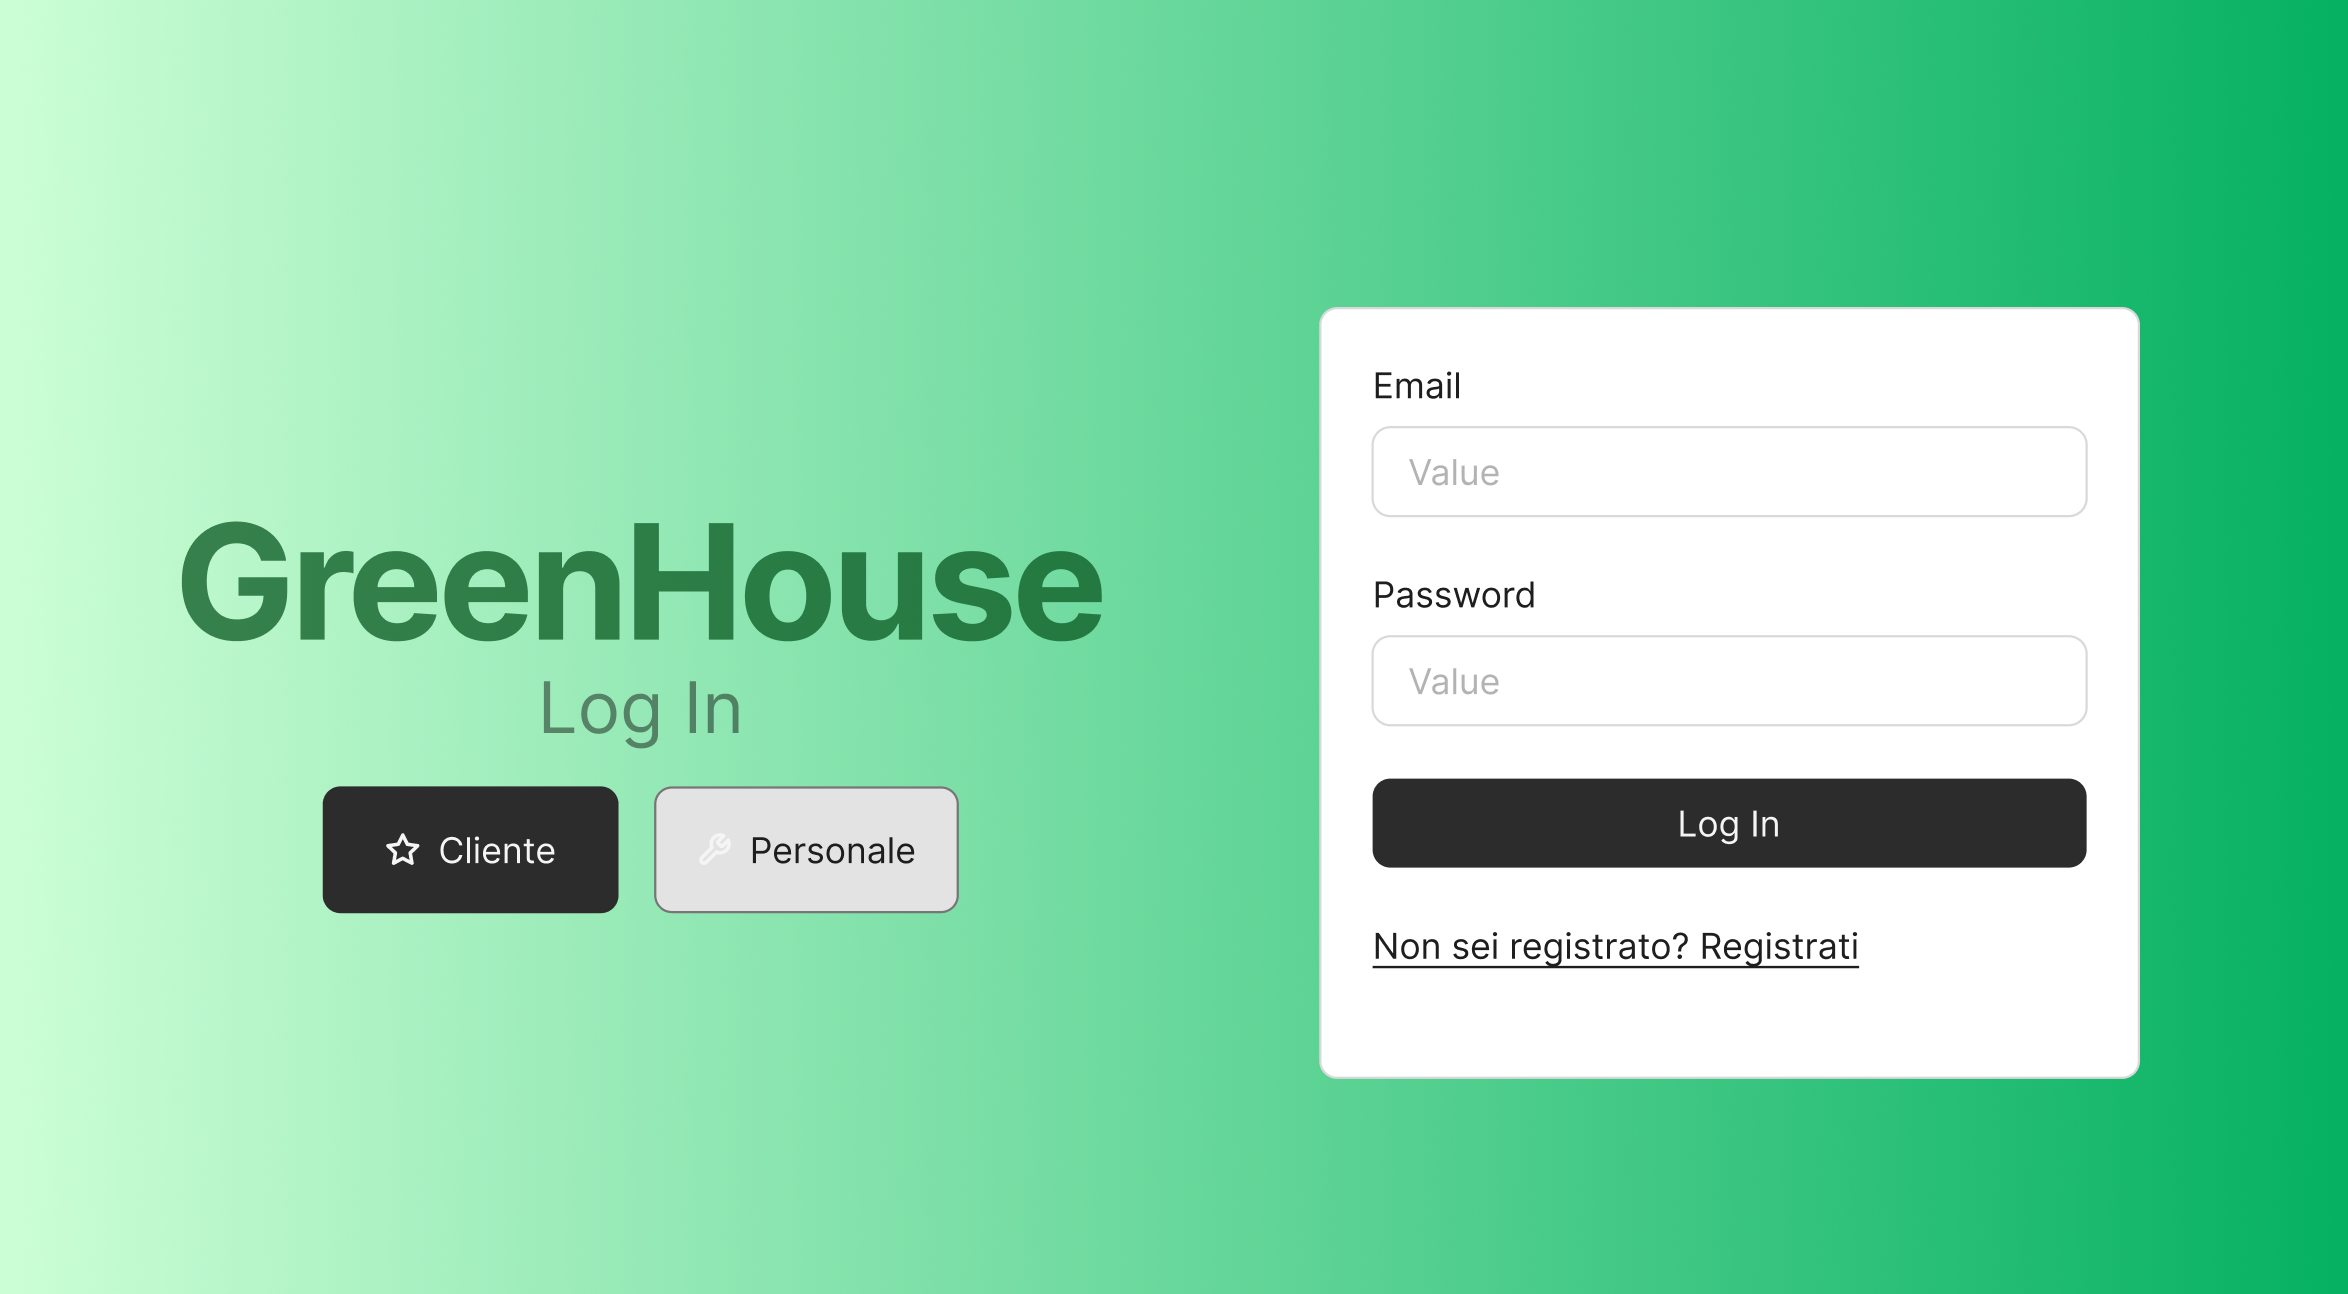
\includegraphics[scale=0.37]{resources/images/Mockups/mockup_1.png}
    \caption{Prototipo della pagina di Sign in - Mockup \#1}
    \label{fig:mockup_1}
\end{figure}
\begin{figure}[H]
    \centering
    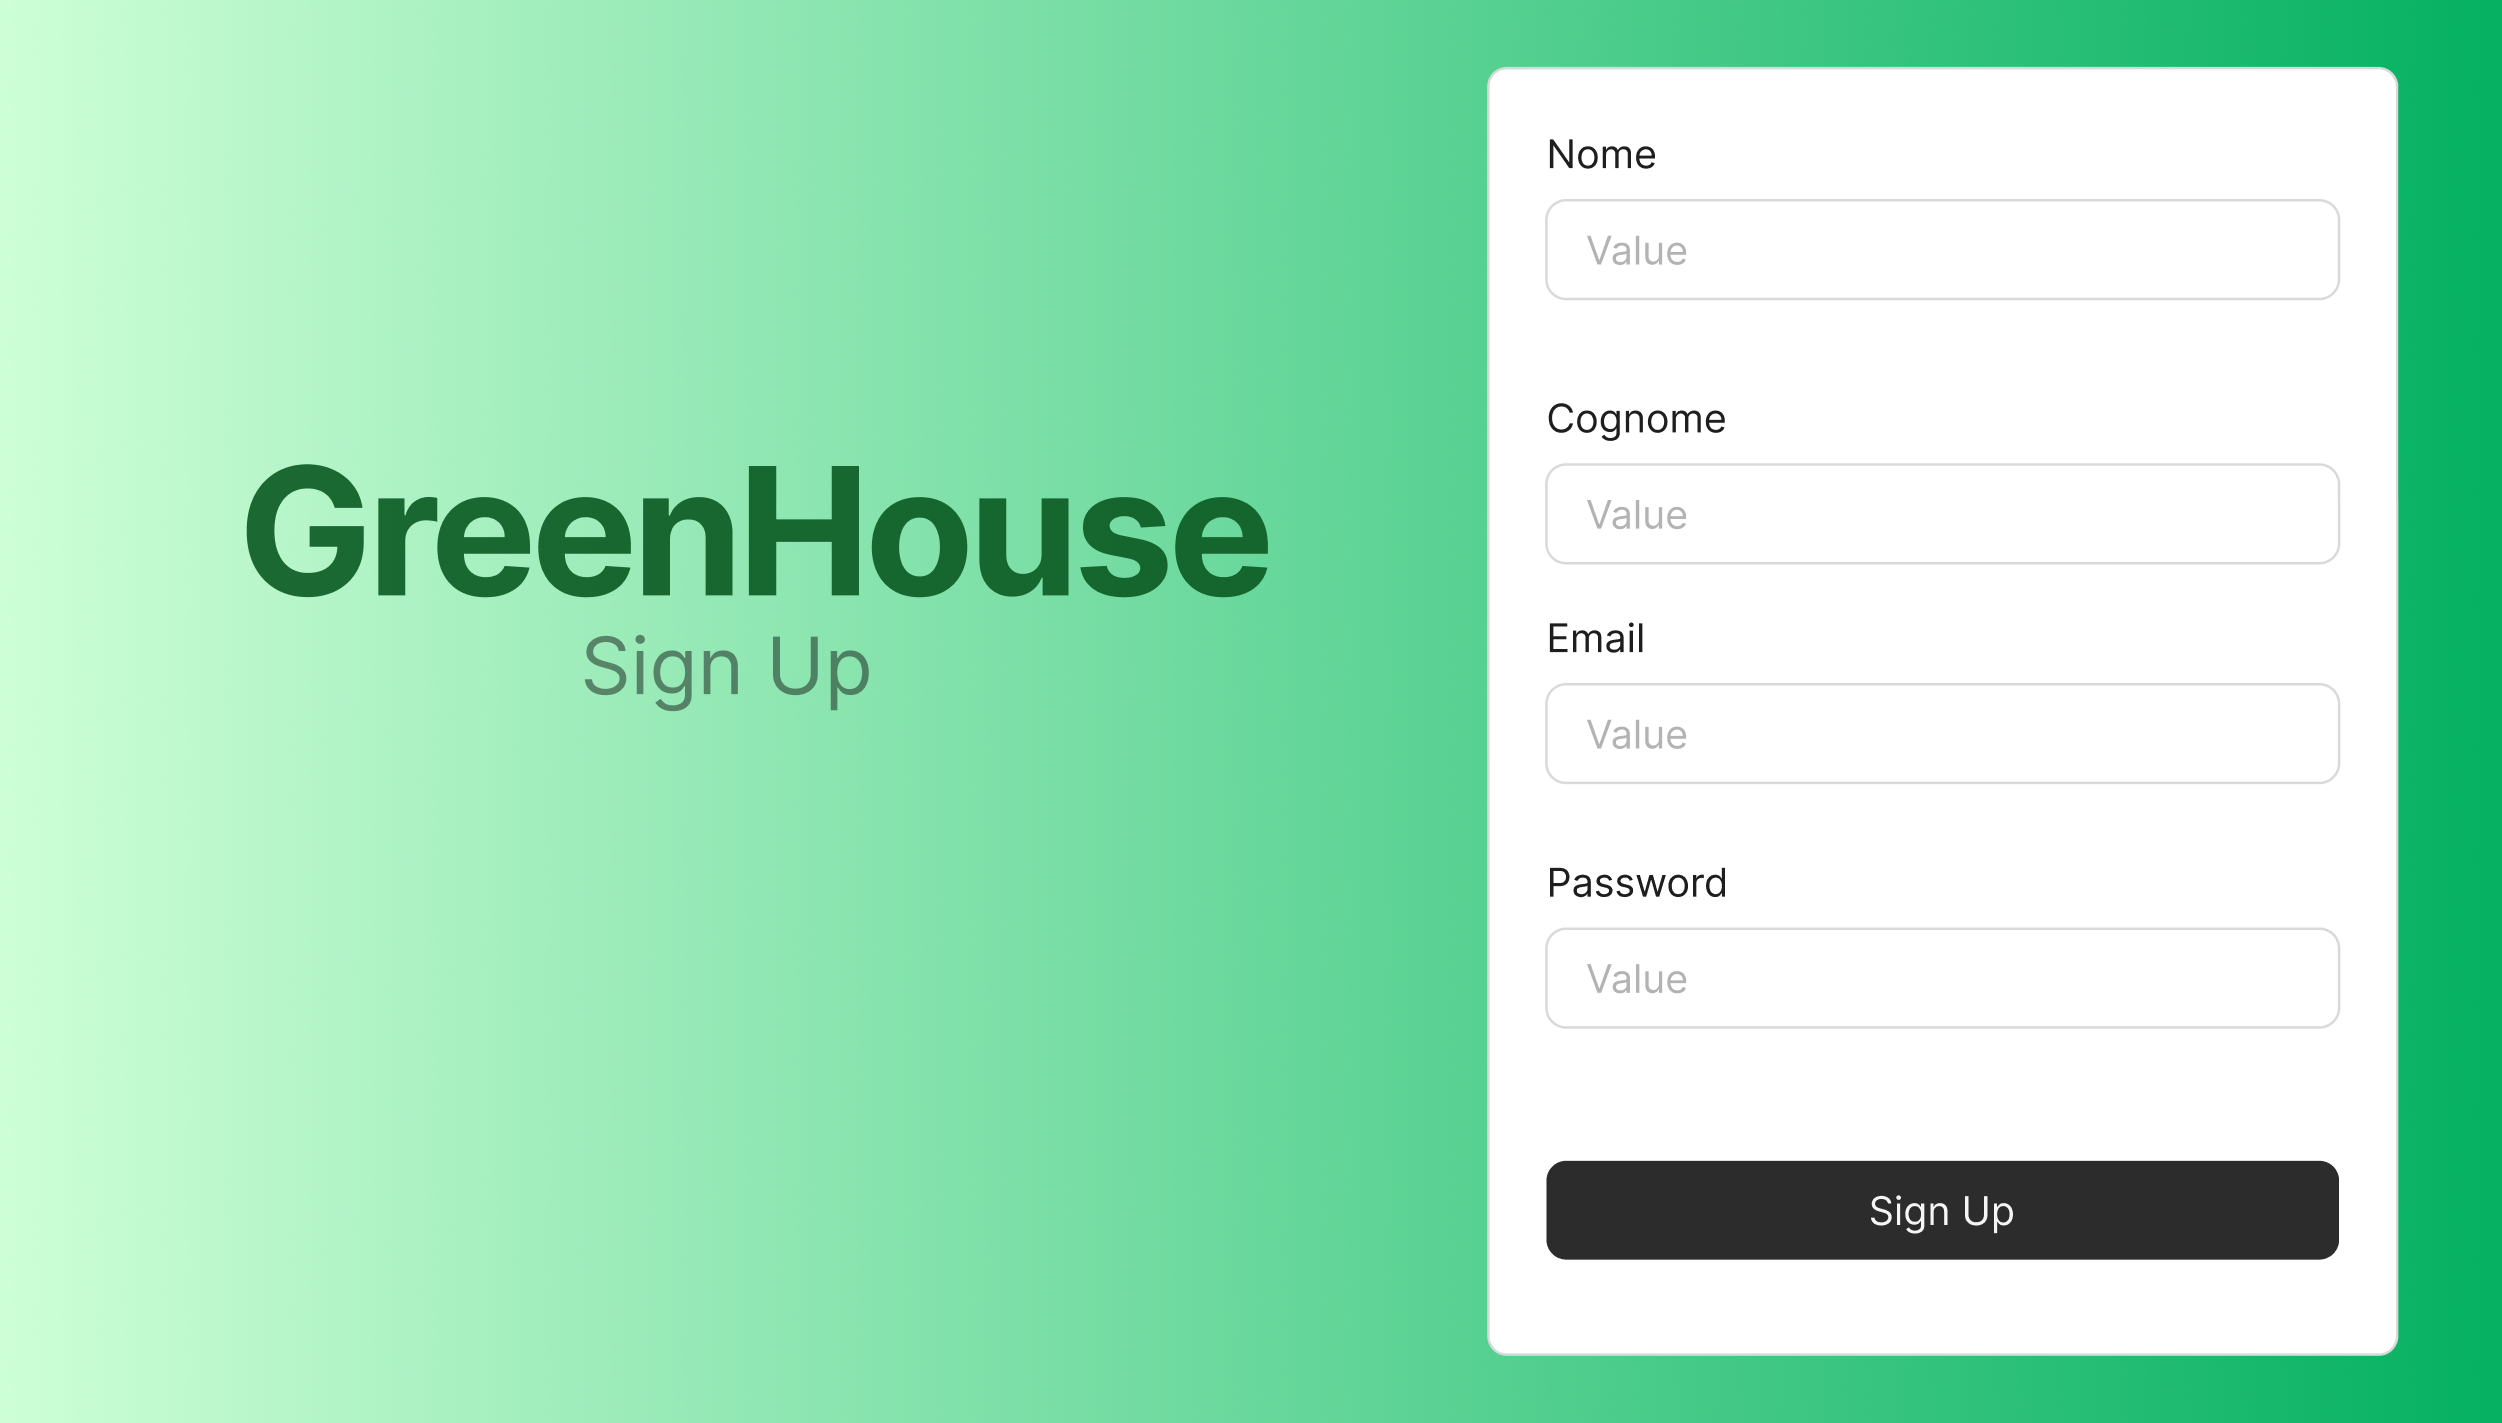
\includegraphics[scale=0.35]{resources/images/Mockups/mockup_2.png}
    \caption{Prototipo della pagina di Sign up - Mockup \#2}
    \label{fig:mockup_2}
\end{figure}
\begin{figure}[H]
    \centering
    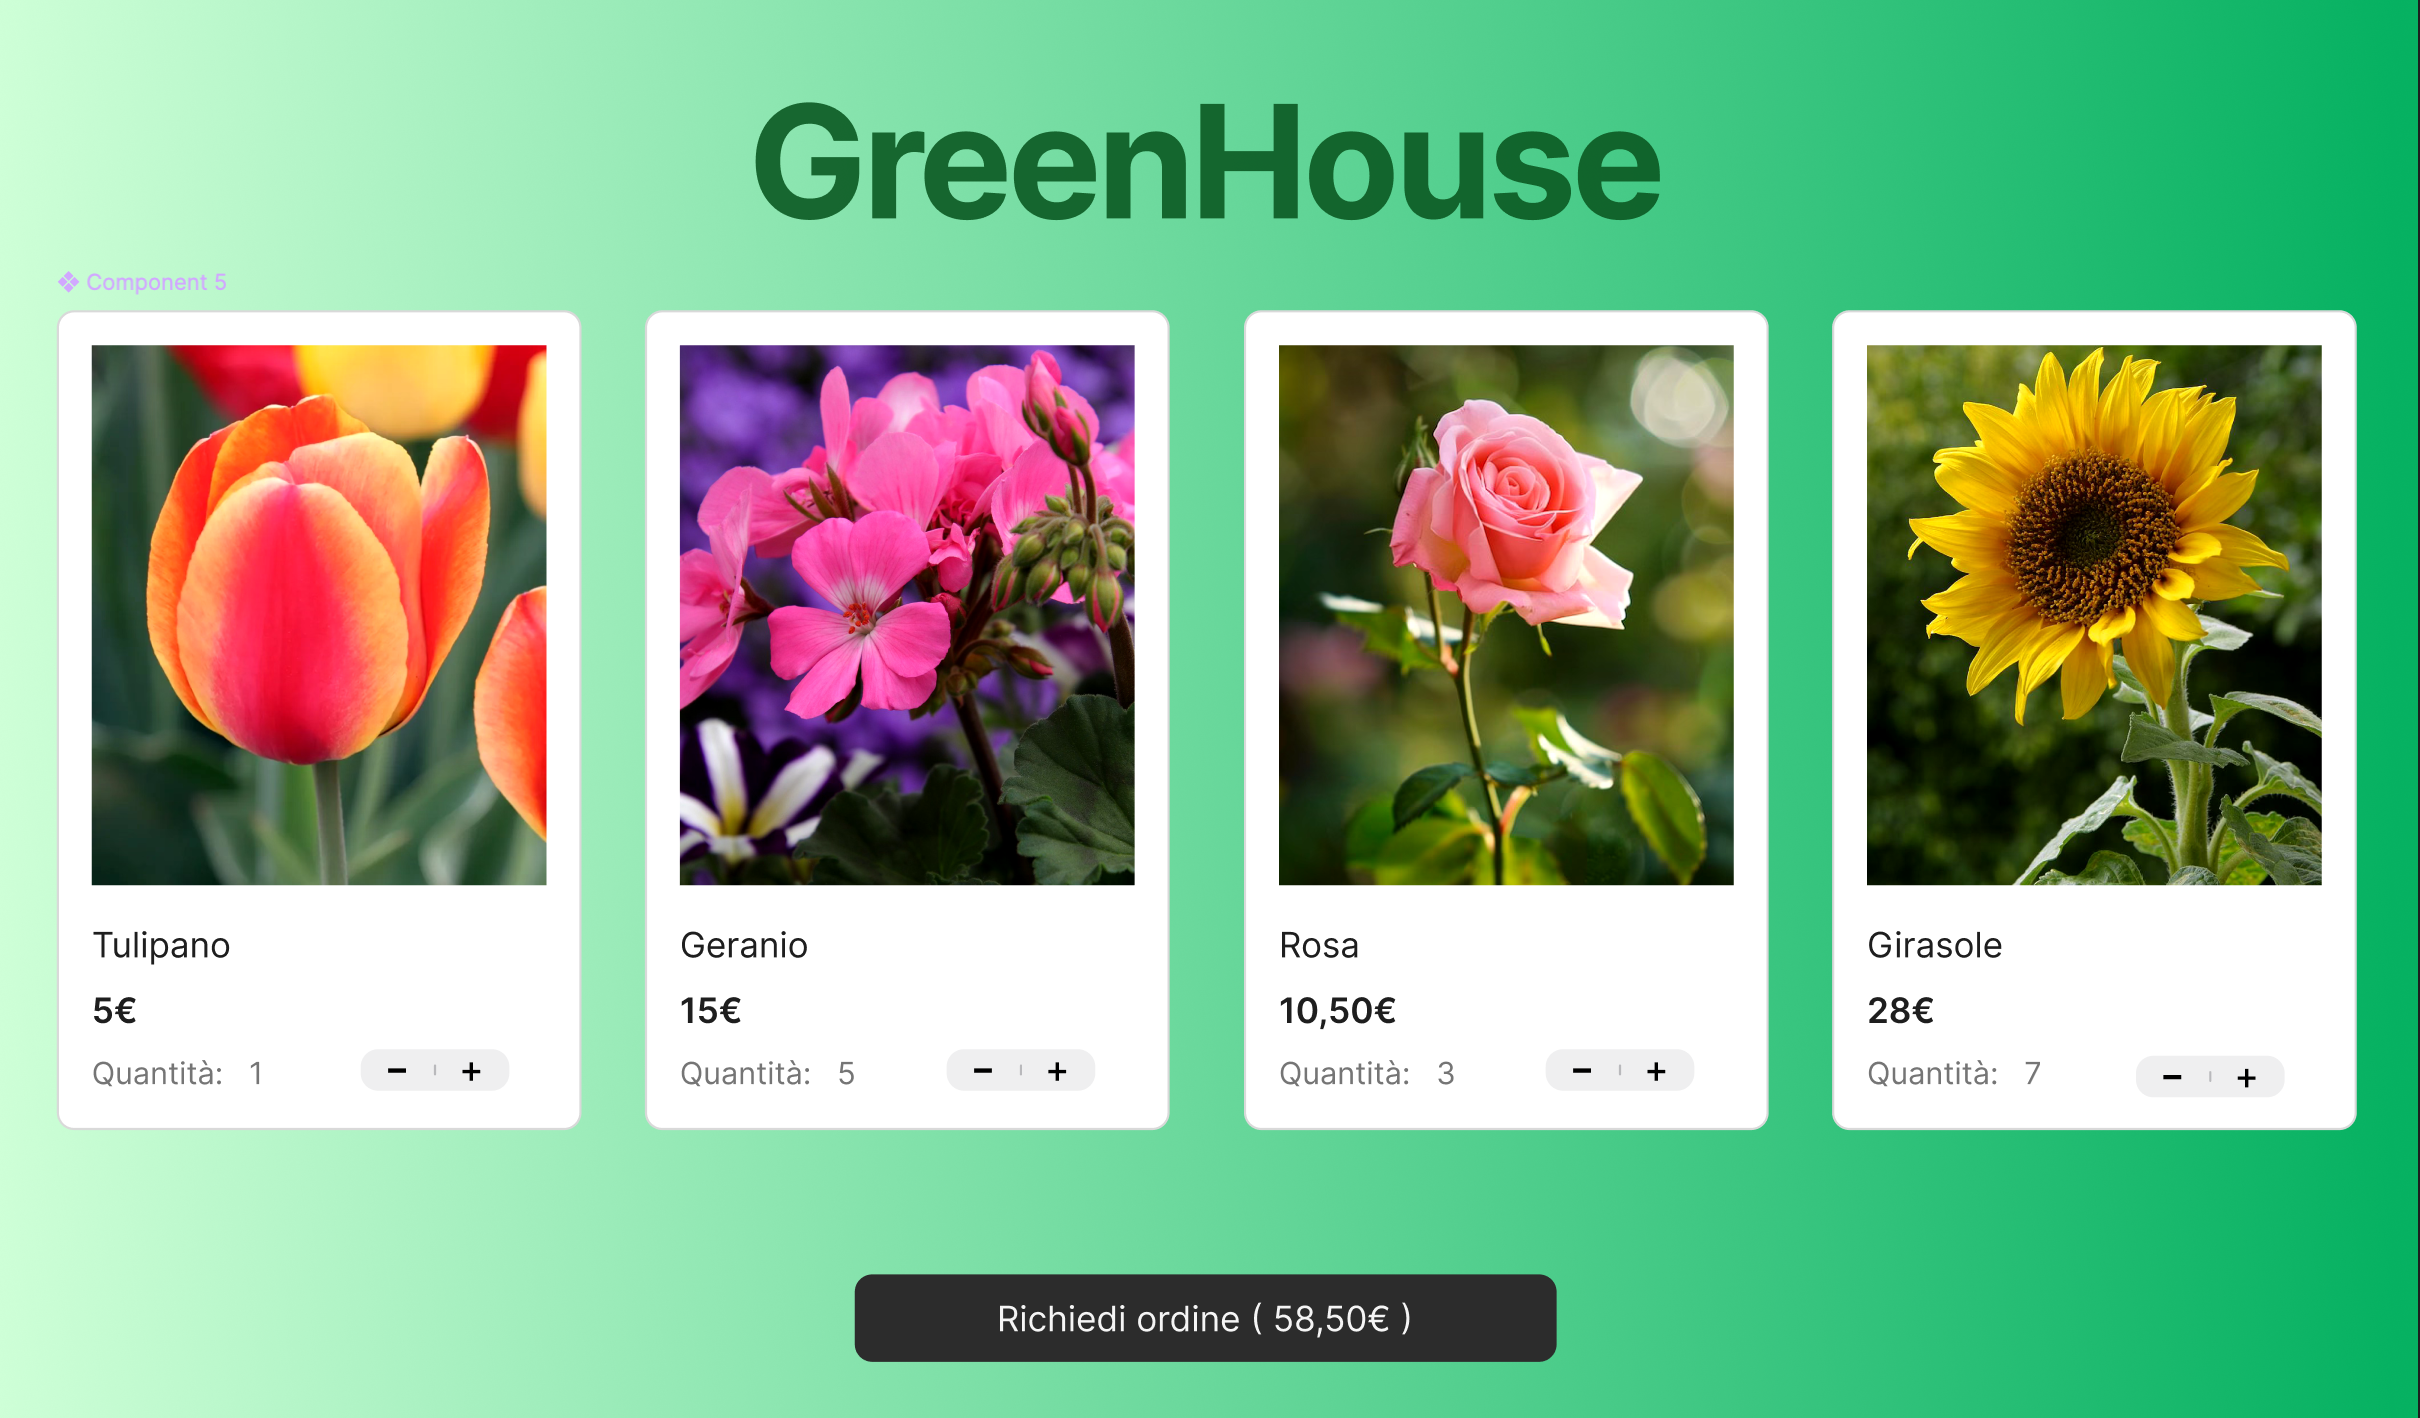
\includegraphics[scale=0.35]{resources/images/Mockups/mockup_3.png}
    \caption{Prototipo della pagina per richiedere nuovi ordini - Mockup \#3}
    \label{fig:mockup_3}
\end{figure}
\begin{figure}[H]
    \centering
    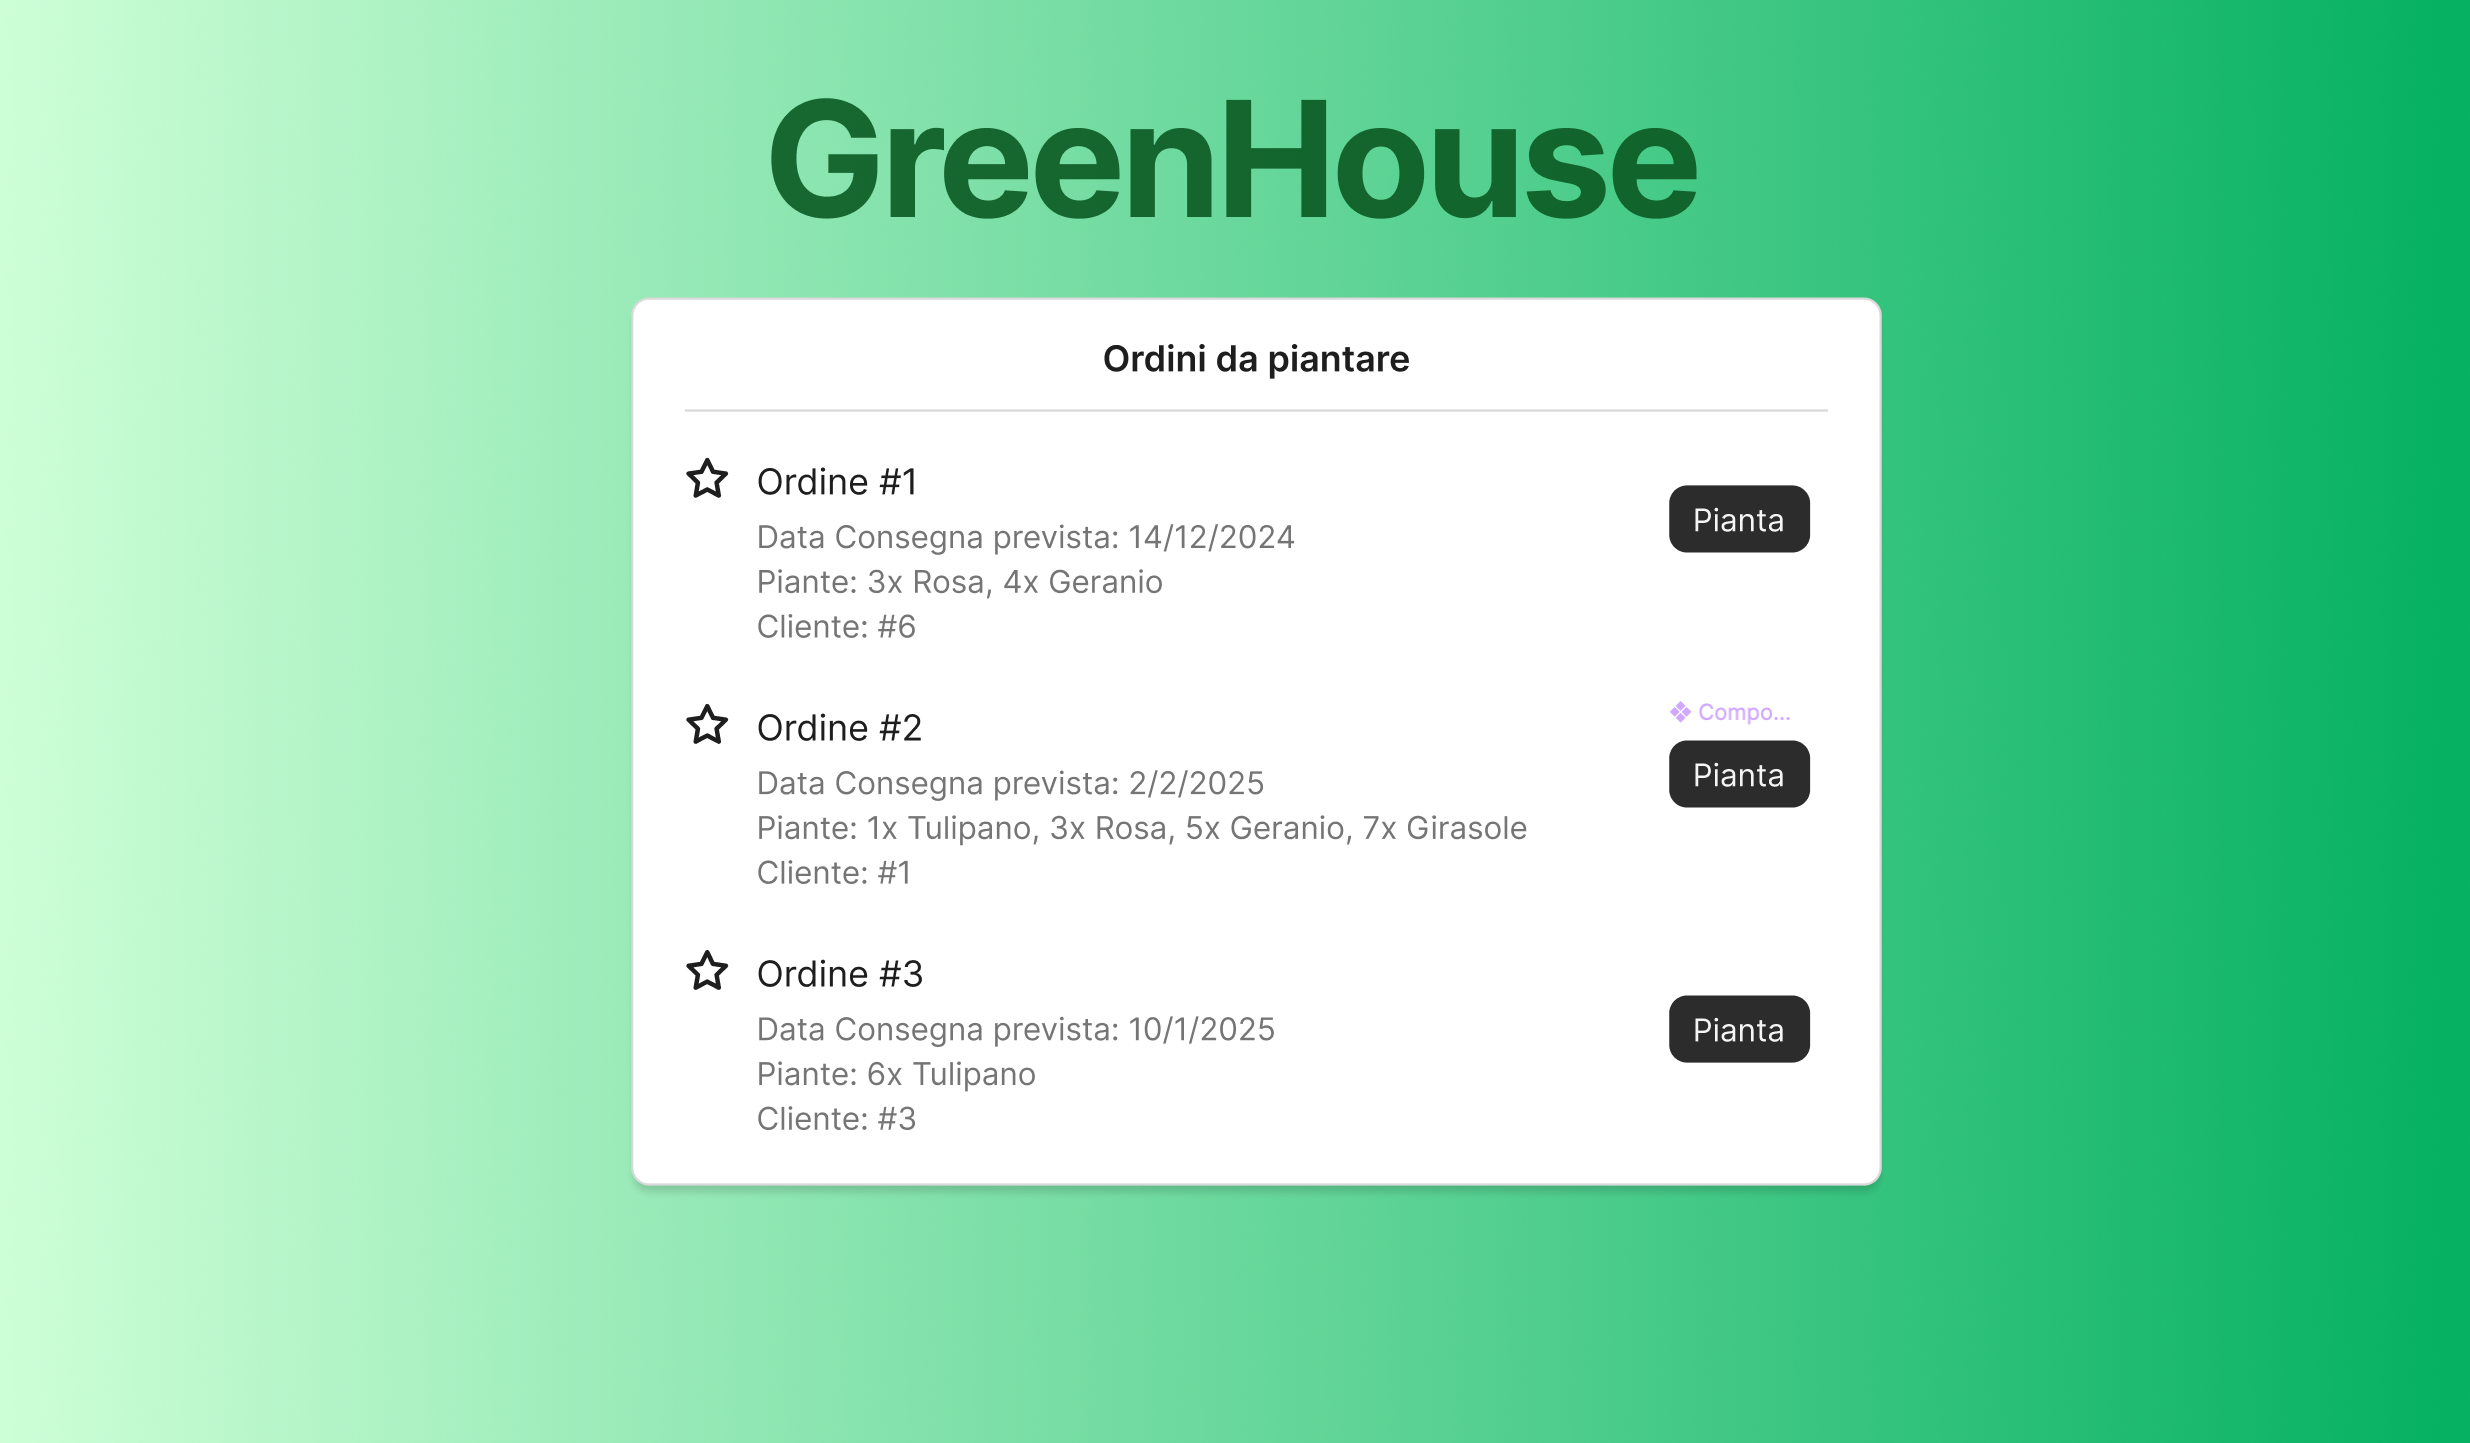
\includegraphics[scale=0.35]{resources/images/Mockups/mockup_4.png}
    \caption{Prototipo della pagina per piantare gli ordini - Mockup \#4}
    \label{fig:mockup_4}
\end{figure}

\subsection{Class Diagram}
Vista la divisione strutturale in 3 packages, sono stati realizzati 3 diagrammi delle classi distinti, uno per ogni package:

\begin{itemize}
    \item \textbf{Business Logic} (Figura \ref{fig:diagram_businesslogic}): contiene le classi che implementano la logica di business del sistema, ovvero i seguenti controller: quello che gestisce l’accesso e la registrazione dei nuovi Clienti (LoginClienteController), degli Admin e degli Operatori (LoginPersonaleController), quello che permette ai Clienti di richiedere nuovi ordini, visualizzarli e di ritirarli (ClienteController), quello che gestisce il monitoraggio e visualizzazione dell'impianto da parte dell'Admin (AdminController), infine il controller che segnala le operazioni dell'operatore come piantare un ordine, completarlo o fare il checkup delle piante (OperatoreController).
    \item \textbf{Domain Model} (Figura \ref{fig:diagram_domainmodel}): contiene le classi che rappresentano le entità del sistema ovvero: Ordine, Utente, Cliente, Operatore, Admin, Pianta e il Posizionamento (quest'ultimo funge da Mapper tra Pianta, Ordine e Posizione). In più contiene anche un altro package chiamato Impianto nel quale sono presenti le classi delle entità che compongono la struttura dell'azienda quali: Spazio, Settore e Settore che ne rappresentano l'entità immobile, Attuatore e Sensori che ne rappresentano le entità operative (nello specifico Climatizzatore, Lampada, Irrigatore sono attuatori; IgrometroAria, IgrometroTerra, Termometro e Fotosensore sono sensori).
    \item \textbf{ORM} (Figura \ref{fig:diagram_orm}): contiene le classi che implementano l’Object-Relational Mapping, quindi contiene una classe per ogni entità del sistema: ClienteDAO, OperatoreDAO, AdminDAO, OrdineDAO, PiantaDAO, PosizionamentoDAO, SettoreDAO, PosizioneDAO, AttuatoreDAO e SensoreDAO. In piu` contiene anche la classe ConnectionManager che si occupa di gestire la connessione al database.
\end{itemize}
\begin{figure}[H]
    \centering
    \fbox{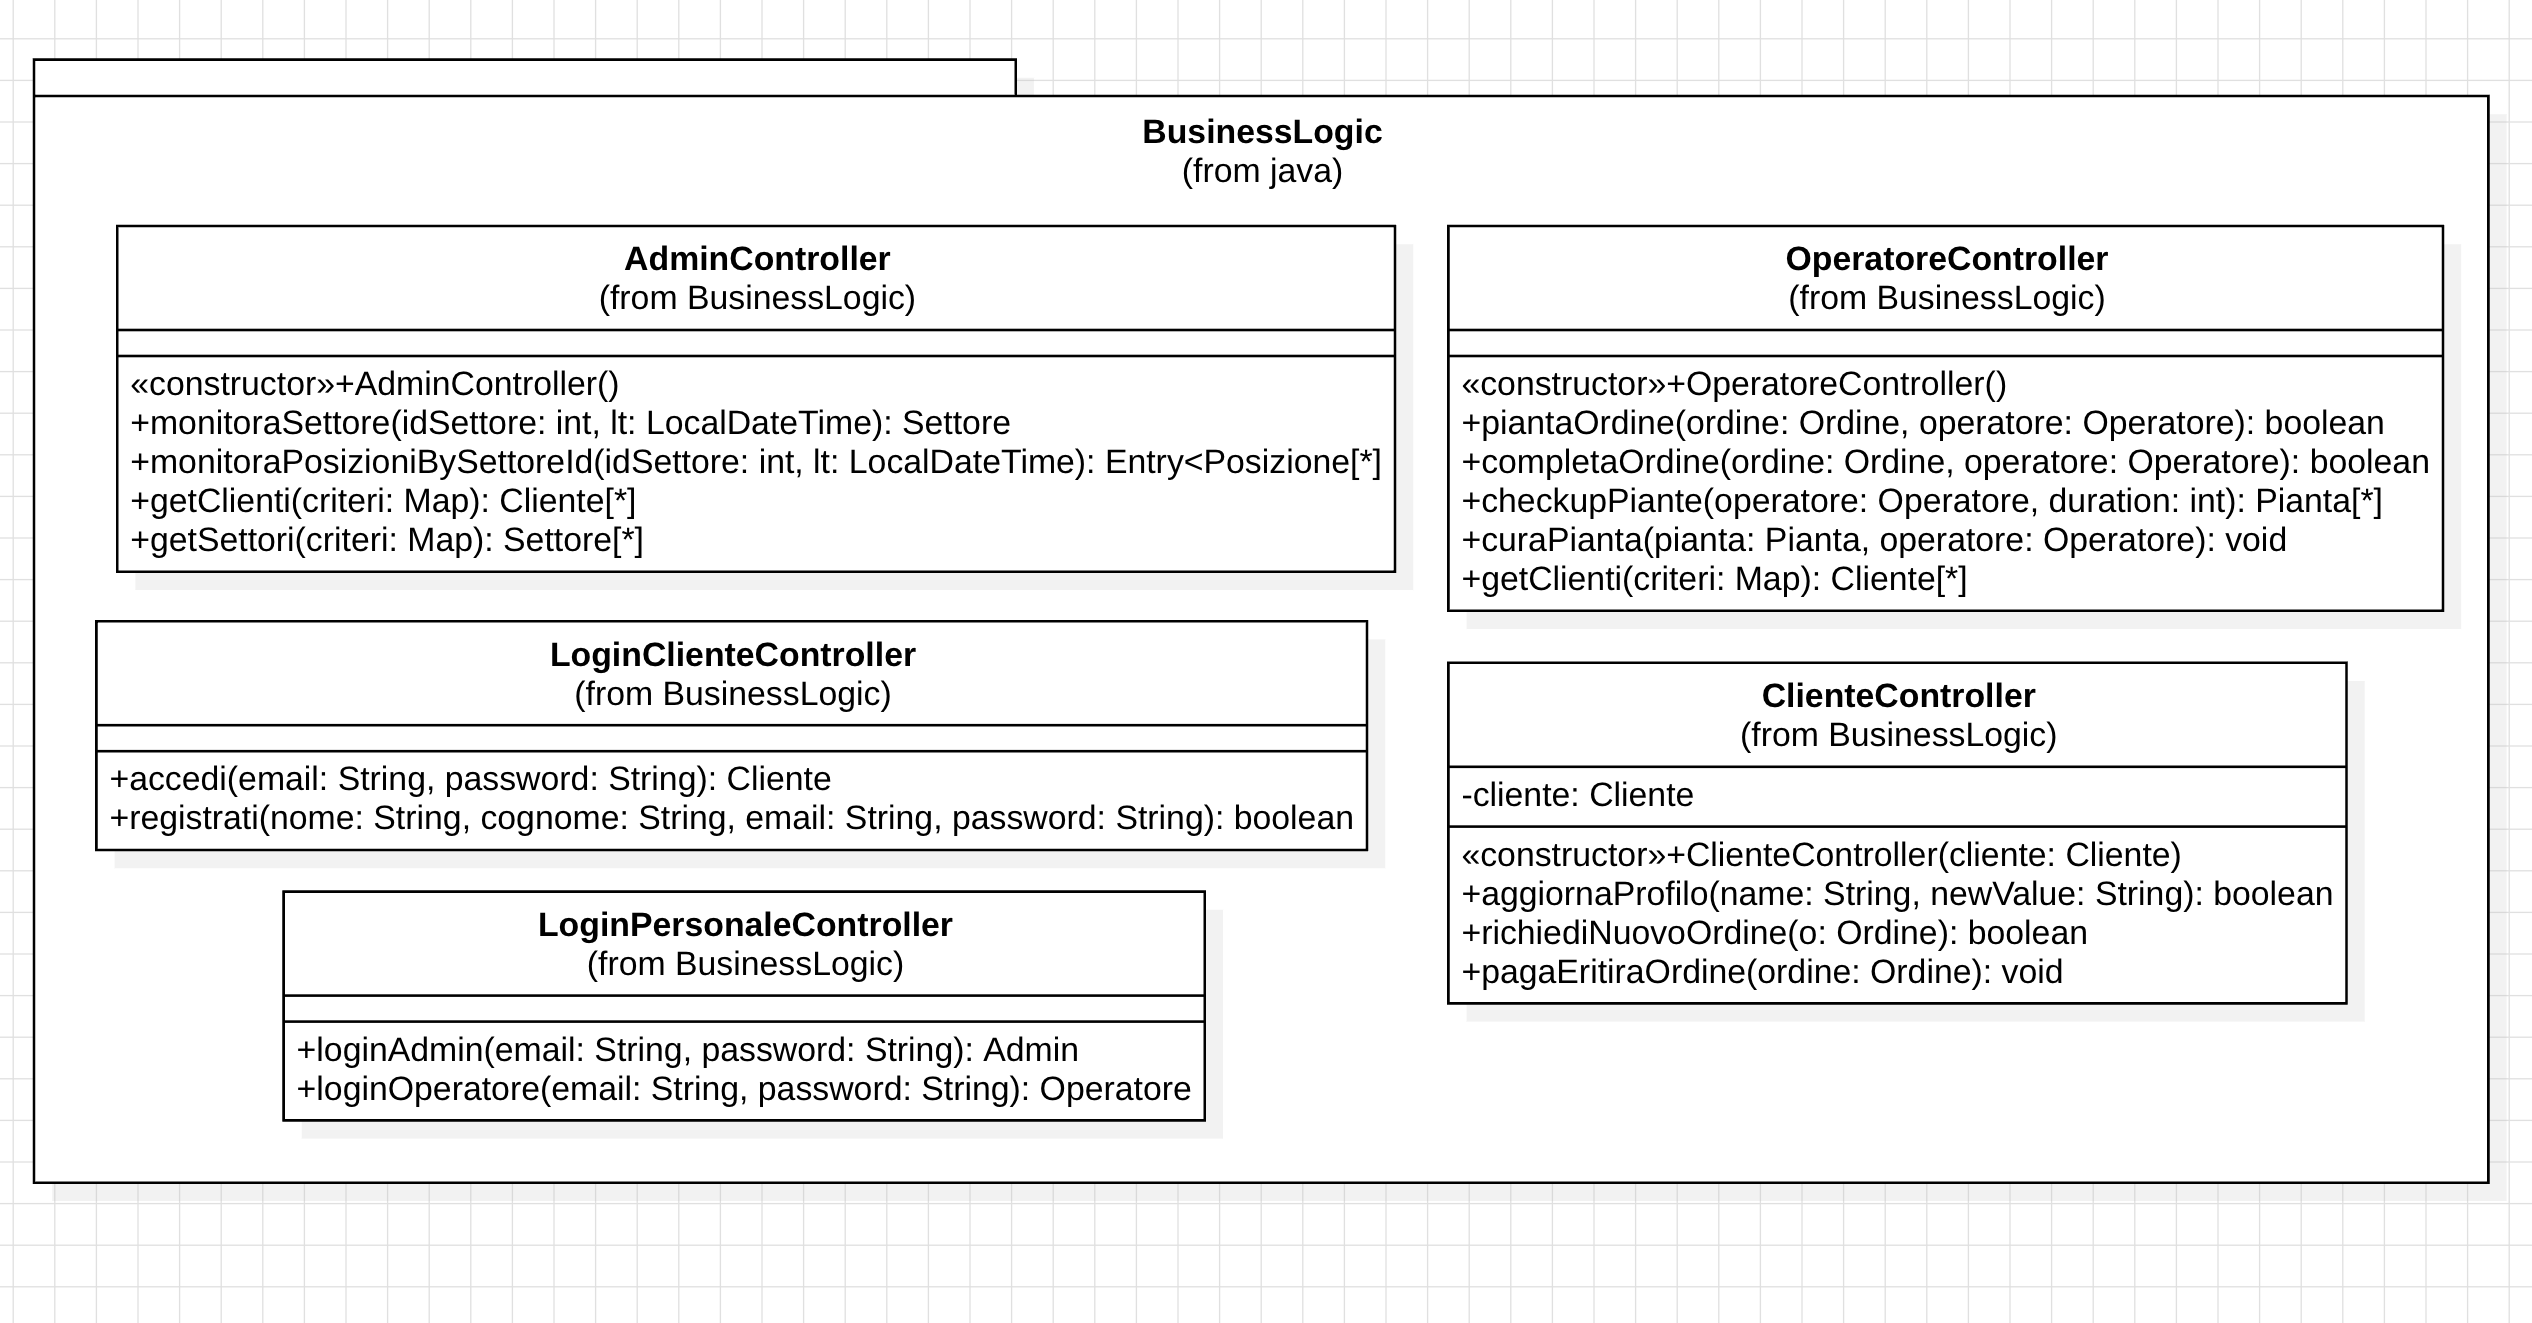
\includegraphics[scale=0.35]{resources/images/Diagrams/diagram_businesslogic.png}}
    \caption{Class Diagram - BusinessLogic}
    \label{fig:diagram_businesslogic}
\end{figure}
\begin{figure}[H]
    \hspace{-1cm}
    \fbox{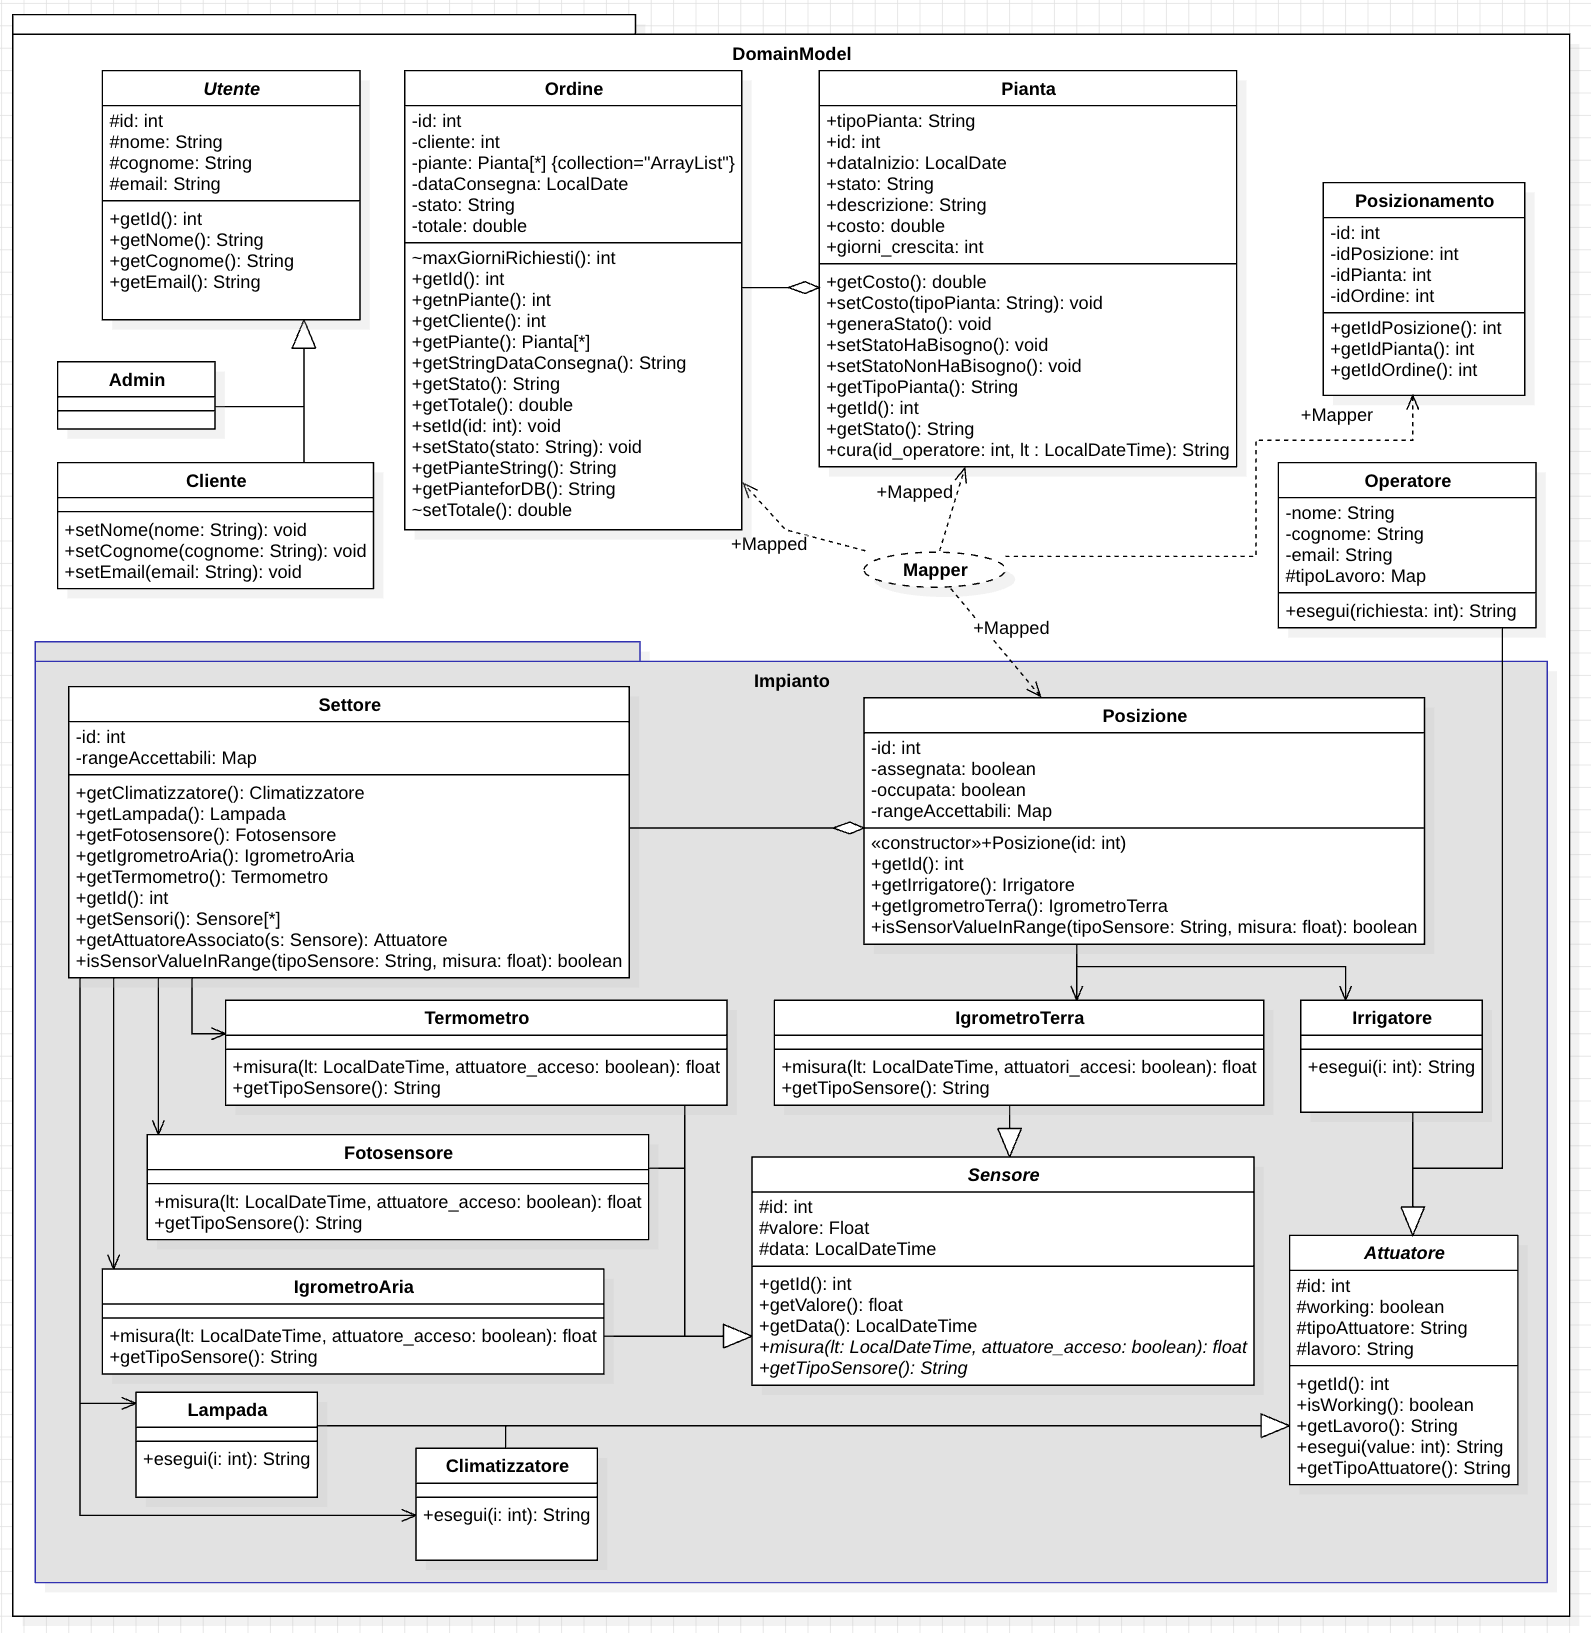
\includegraphics[scale=0.62]{resources/images/Diagrams/diagram_domainmodel.png}}
    \caption{Class Diagram - DomainModel}
    \label{fig:diagram_domainmodel}
\end{figure}
\begin{figure}[H]
    \centering
    %\hspace{-1.7cm}
    \fbox{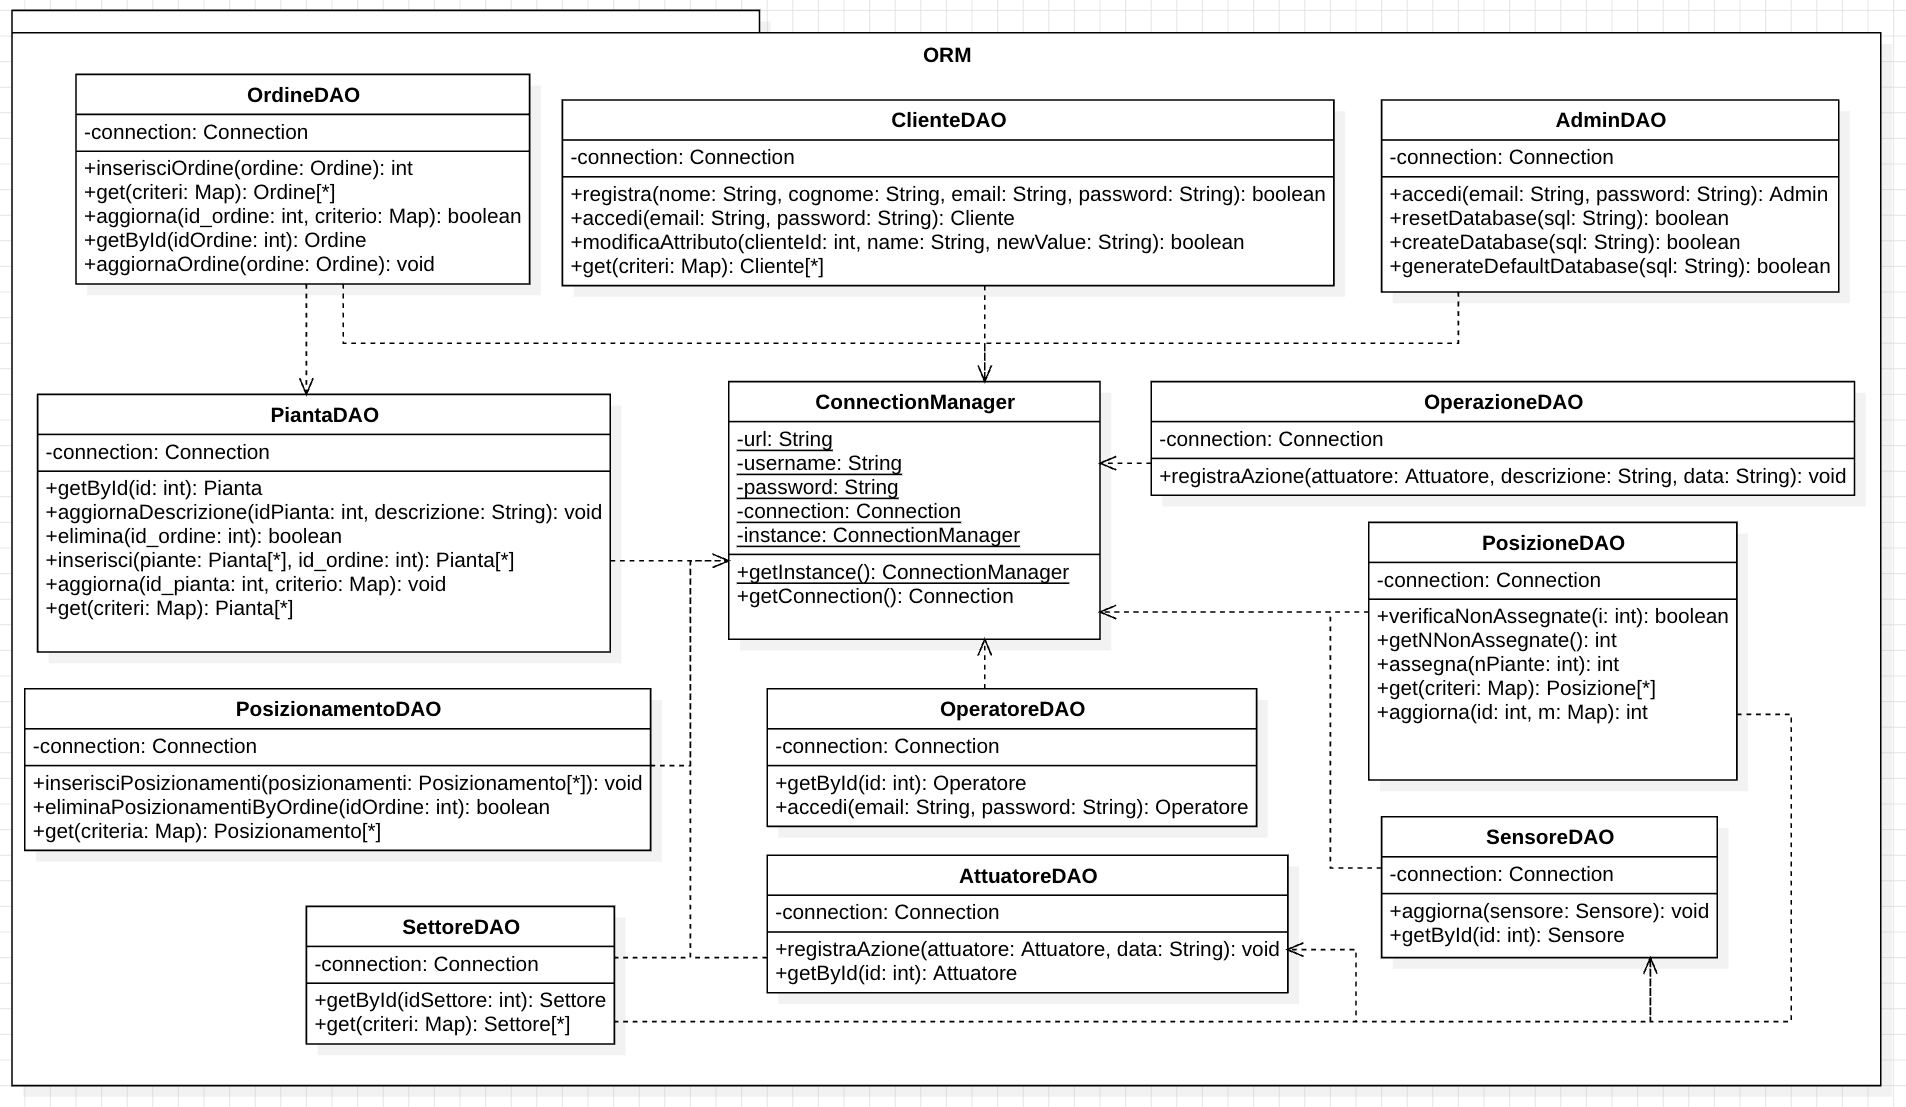
\includegraphics[scale=0.5]{resources/images/Diagrams/diagram_orm.png}}
    \caption{Class Diagram - ORM}
    \label{fig:diagram_orm}
\end{figure}
\subsection{ER Diagram e modello relazionale}
Il database è stato progettato seguendo il modello relazionale e facendo attenzione alle relazioni che legano le entità (Figura \ref{fig:diagram_er}).\\
Sono state quindi definite le seguenti tabelle:
\begin{itemize}
    \item \textbf{Cliente}: rappresenta l'entità Cliente;
    \item \textbf{Ordine}: rappresenta l’entità Ordine e risolve la relazione "richiedi" con Cliente (un Cliente può fare più Ordini, quindi gli Ordini contengono l'id del Cliente che li ha effettuati);
    \item \textbf{Pianta}: rappresenta l’entità Pianta e risolve la relazione "ha" con Ordine, in quanto un Ordine possiede un insieme di Piante, quindi ogni pianta possiede l'id dell'Ordine a cui appartiene;
    \item \textbf{Admin}: rappresenta l’entità Admin;
    \item \textbf{Operatore}: rappresenta l’entità Operatore;
    \item \textbf{Spazio}: rappresenta l’entità Spazio;
    \item \textbf{Settore}: rappresenta l’entità Settore e contiene l'id dello Spazio a cui appartiene, e gli id dei Sensori e degli Attuatori situati in esso (relazioni di appartenenza);
    \item \textbf{Posizione} rappresenta l’entità Posizione, prende parte alla relazione "Posizionamento" e contiene gli id dei sensori e attuatori che gli appartengono;
    \item \textbf{Posizionamento}: rappresenta l’entità Posizionamento che risolve la relazione di mapping tra Ordine, Pianta e Posizione;
    \item \textbf{Attuatore}: rappresenta l’entità Attuatore.
    \item \textbf{Sensore}: rappresenta l’entità Sensore.
    \item \textbf{Operazione}: rappresenta l’entità Operazione;
\end{itemize}
\begin{figure}[H]
    \centering
    \fbox{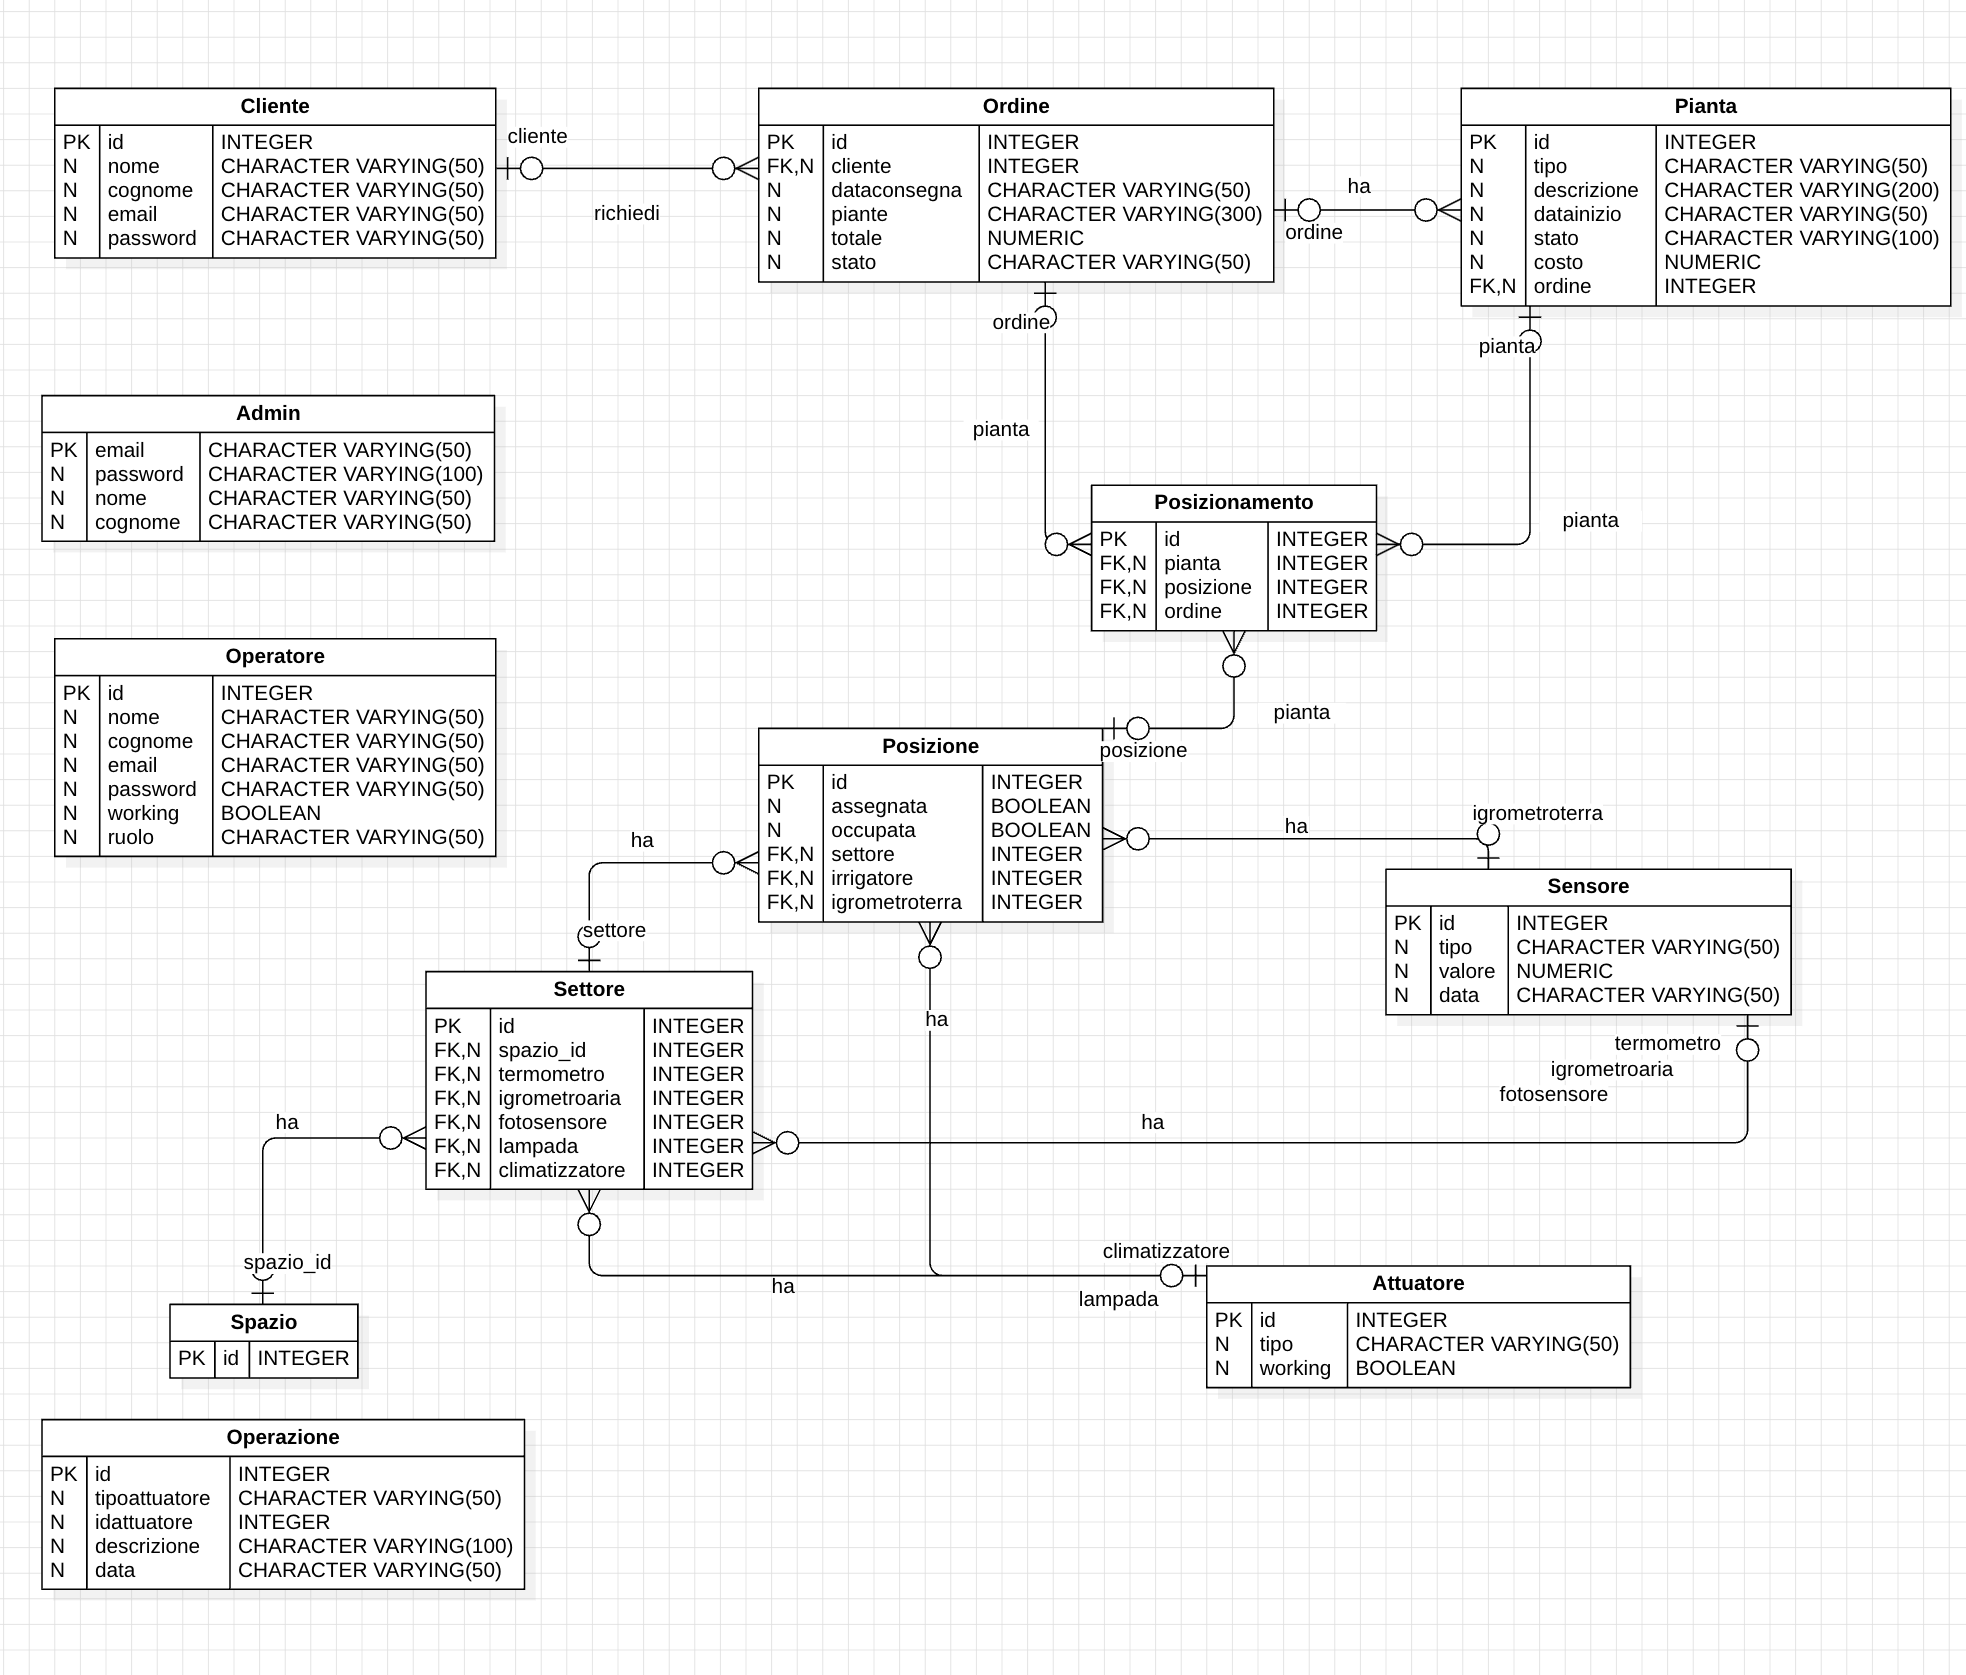
\includegraphics[scale=0.4]{resources/images/Diagrams/diagram_er.png}}
    \caption{ER Diagram}
    \label{fig:diagram_er}
\end{figure}

\begin{figure}[H]
    \centering
    \fbox{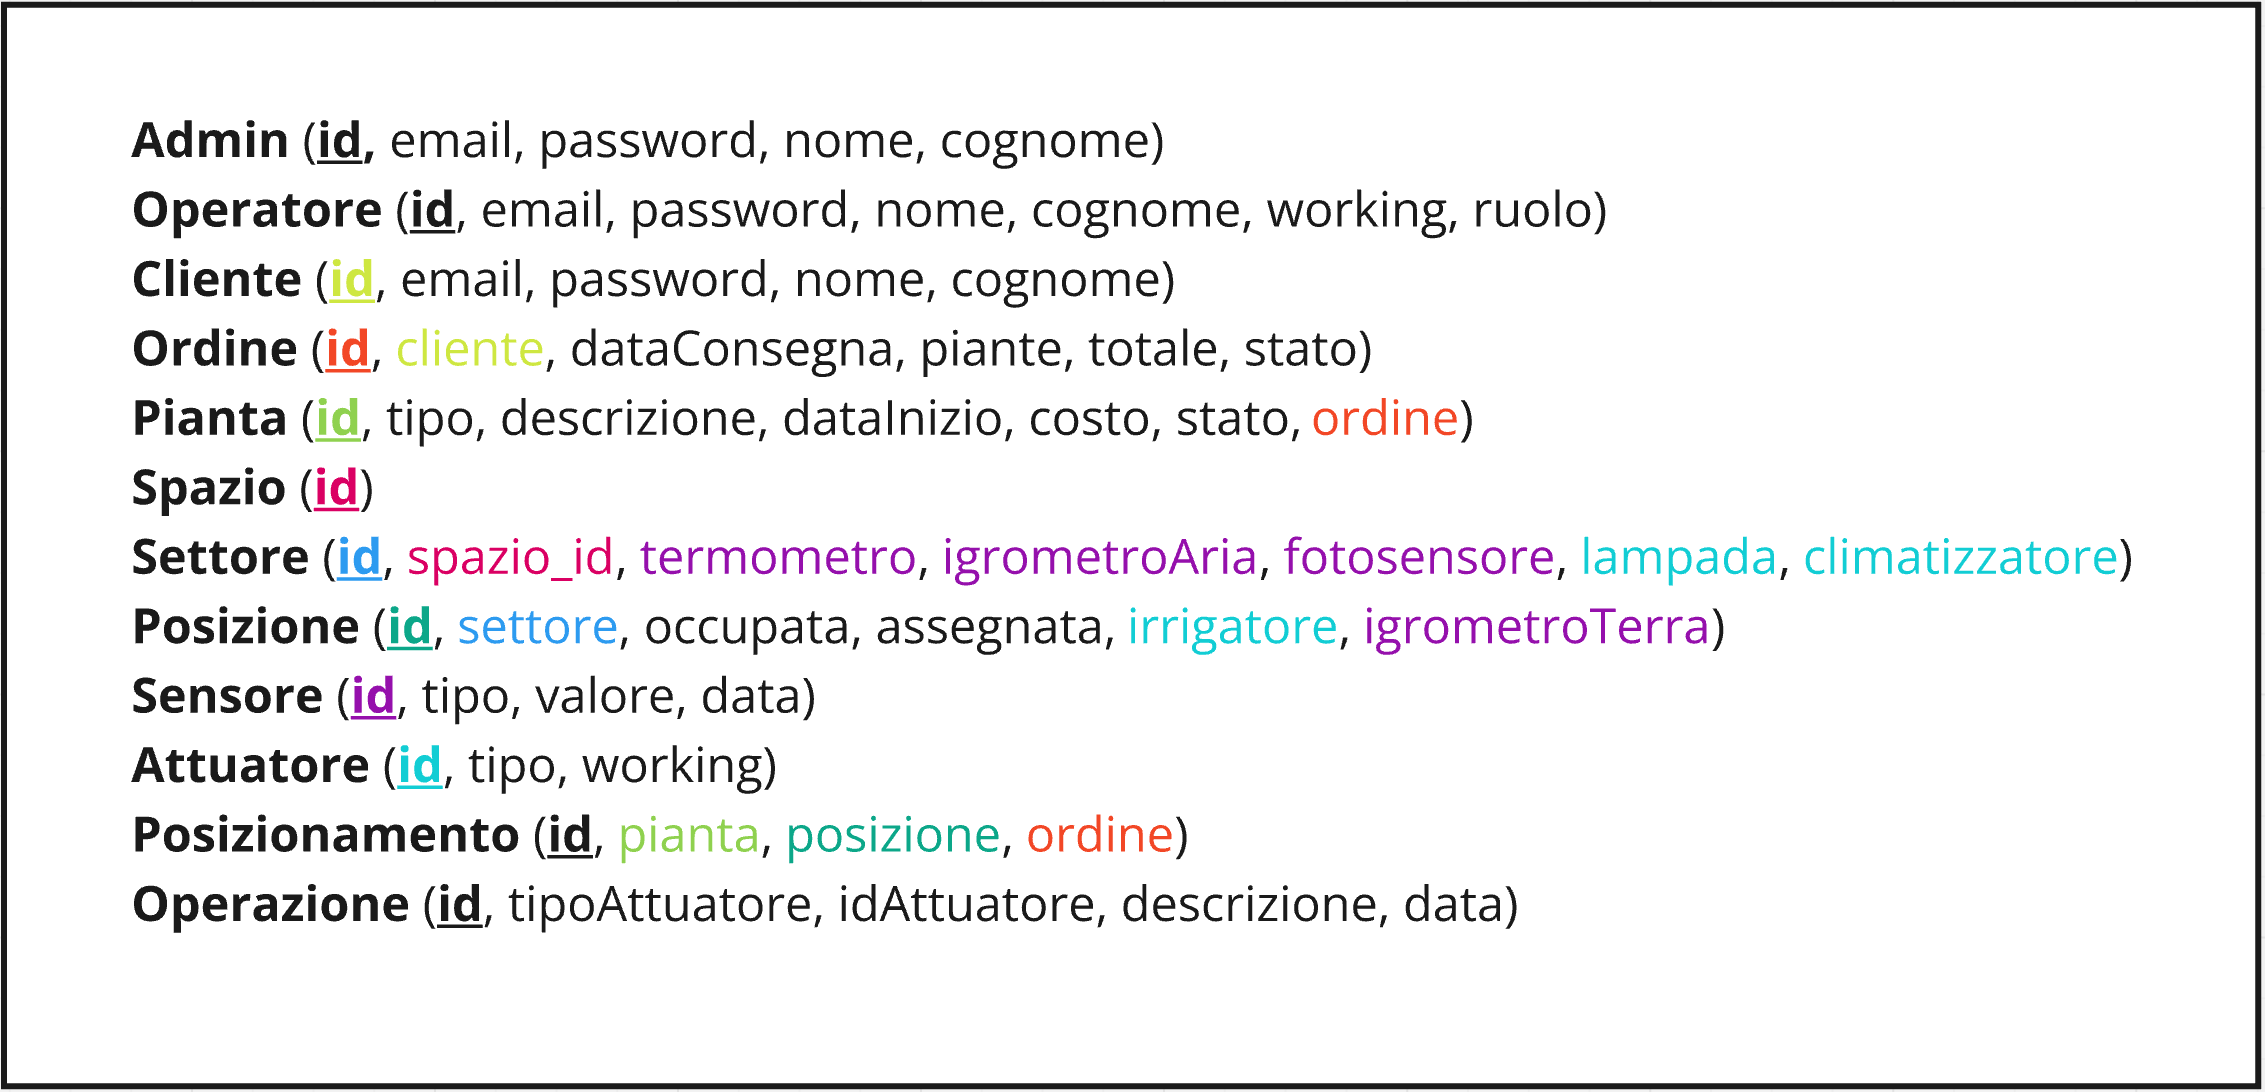
\includegraphics[scale=0.3]{resources/images/Diagrams/diagram_modellorelazionale.png}}
    \caption{Modello Relazionale}
    \label{fig:diagram_modellorelazionale}
\end{figure}

\subsection{Navigation Diagram}
\label{subsec:nav-diagram}
Il seguente diagramma (Figura \ref{fig:diagram_navigation}) rappresenta quelle che sono le pagine principali del sistema e le possibili azioni che l’utente può compiere. Sono anche rappresentati i modi con cui si può navigare tra le varie pagine.
Alcune delle pagine sono:
\begin{itemize}
    \item \textbf{Greenhouse}: l'utente sceglie la propria area di appartenenza.
    \item \textbf{Cliente Dashboard}: il cliente può scegliere se entrare nella pagina degli Ordini e quindi crearne uno nuovo, pagarne uno pronto o controllarli, oppure nella pagina Profilo dove può visualizzare o modificare i dati del proprio profilo.
    \item \textbf{Operatore Dashboard}: L'operatore può eseguire i suoi compiti tra quelli elencati quindi piantare un ordine, completarlo per poter essere ritirato dal cliente oppure può eseguire un controllo sullo stato delle piante.
    \item \textbf{Admin Dashboard}: L'admin ha come funzione principale quella di monitorare i settori e le relative posizioni occupate grazie ai sensori e attuatori. Inoltre può visualizzare, come l'operatore, le tabelle di ordini, piante e clienti.
\end{itemize}
\begin{figure}[H]
    \centering
    \fbox{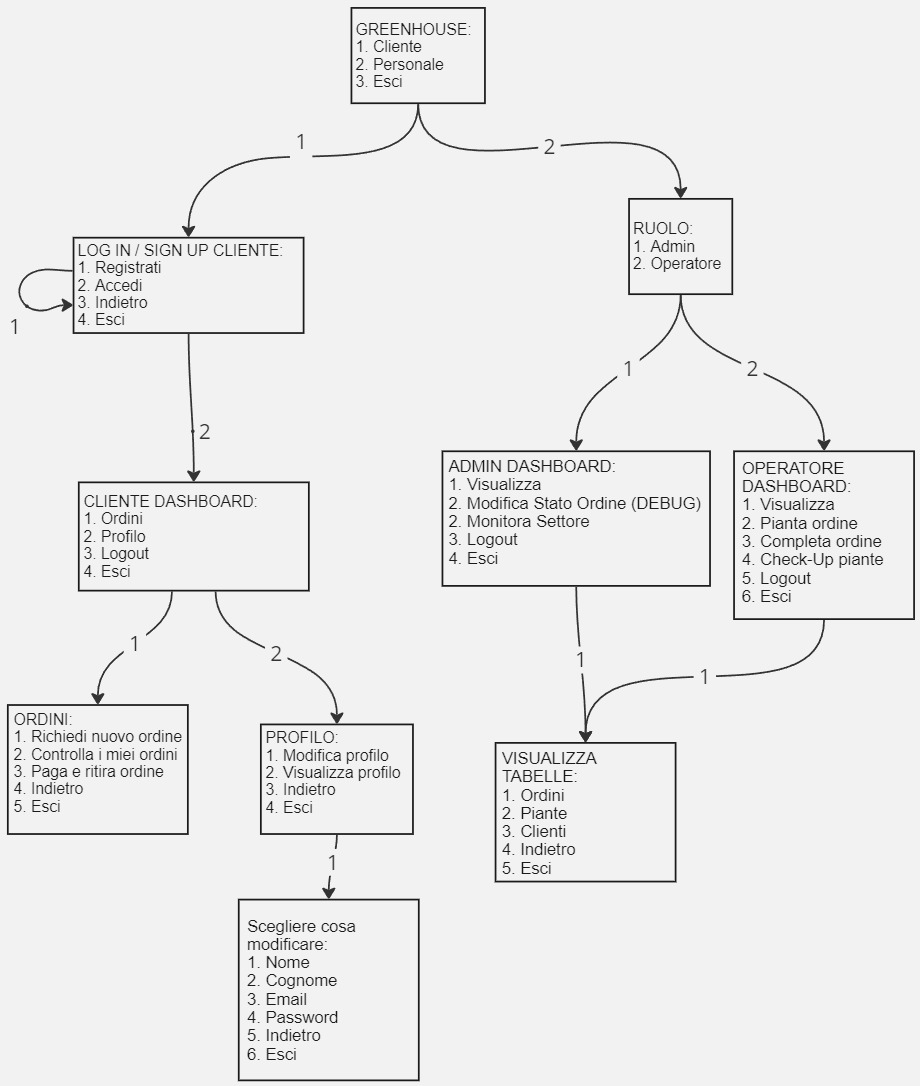
\includegraphics[scale=0.4]{resources/images/Diagrams/diagram_navigation.jpg}}
    \caption{Navigation Diagram}
    \label{fig:diagram_navigation}
\end{figure}


\section{Implementazione}
Il codice è suddiviso in 3 "packages", che suddividono le classi in base alle loro funzionalità:

\subsection{Domain Model}
Contiene tutte le classi che rappresentano le entità del sistema e le relative funzioni associate.

\subsubsection{Utente}
La classe astratta Utente rappresenta un utente del sistema. 
Qui di seguito sono elencate le 3 classi che ereditano Utente e rappresentano gli agenti reali che accedono e interagiscono con il sistema stesso.

\begin{itemize}
    \item \textbf{Cliente:}
    Rappresenta un Cliente dell'azienda, interessato a effettuare un acquisto di piante su ordinazione. I campi della classe sono \code{id}, \code{nome}, \code{cognome}, \code{email} e \code{password}.

    \item \textbf{Admin:} Identifica l'Admin dell'azienda e, come \code{Cliente}, contiene \code{id}, \code{nome}, \code{cognome}, \code{email} e \code{password}. 
    La sua interfaccia gli permette di visualizzare ordini, piante e clienti e monitorare i settori dell'impianto.

    \item \textbf{Operatore:}
    Rappresenta un \code{Operatore} che lavora nell'azienda. È un utente, che quindi può accedere con le proprie credenziali, come un Utente qualsiasi, però può essere visto anche come un Attuatore con più funzionalità. Infatti può piantare un ordine, prepararlo quando è pronto oppure può controllare lo stato delle piante. I suoi attributi sono \code{id, nome, cognome, email, password e working}.
\end{itemize}

\subsubsection{Pianta}
    Rappresenta una \code{pianta} presente nella serra, viene definita con \code{tipo di Pianta}, una \code{descrizione} di essa, la \code{dataInizio} in cui è stata piantata, lo \code{stato} attuale, il suo \code{costo} e il numero di \code{giorni} necessari alla sua crescita.\\
    Il metodo \code{cura} effettua una cura (simulata) da parte di un Operatore nel caso in cui la Pianta ne necessiti.
    
\subsubsection{Ordine}
    Identifica un \code{ordine} di certe \code{piante} effettuato da un \code{cliente} e i relativi dettagli come la \code{data di consegna}, il prezzo \code{totale}, un \code{id} univoco e lo \code{stato} attuale.
    I suoi metodi sono tutti getters e setters.\\
    Lo \code{stato} dell'Ordine può essere:
    \begin{itemize}
        \item "da piantare": l'ordine è stato accettato dal sistema ed è stato preso in carico;
        \item "posizionato": le piante richieste nell'ordine sono state seminate nelle posizioni;
        \item "da completare": le piante sono cresciute e sono pronte per essere tolte dalle posizioni;
        \item "da ritirare": le piante possono essere ritirate dal cliente;
        \item "ritirato": l'ordine è stato pagato e ritirato dal cliente.
    \end{itemize}
    I passaggi di stato sono attuati attraverso precise funzioni del sistema (vedi Figura \ref{fig:diagram_statiordine}). In particolare \code{modificaStatoOrdine} permette di impostare uno stato arbitrario ed è utilizzata esclusivamente per "debug", però è indispensabile dato che la parte di simulazione della crescita della pianta e quindi del passaggio dell'ordine a stato "da completare" non è stata implementata.

    \begin{figure}[H]
        \centering
        \fbox{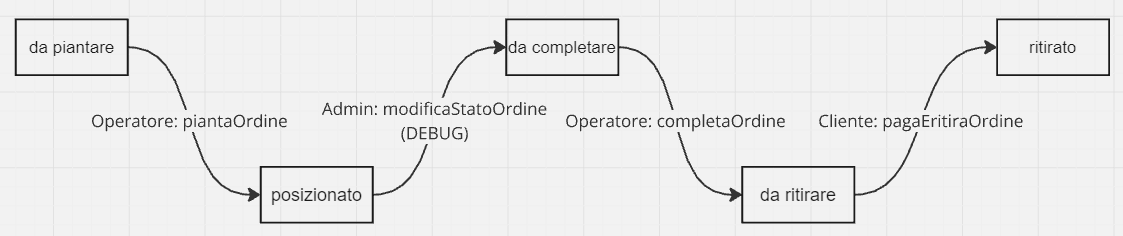
\includegraphics[scale=0.5]{resources/images/Diagrams/diagram_statiordine.png}}
        \caption{Diagramma degli Stati di un Ordine}
        \label{fig:diagram_statiordine}
    \end{figure}


\subsubsection{Impianto}
\begin{itemize}
    \item \textbf{Spazio:}
    Rappresenta uno \code{Spazio} presente nella GreenHouse.
    È identificato da un \code{id} e contiene un insieme di Settori.
    \item \textbf{Settore:} Rappresenta una zona chiusa e isolata (fisicamente) avente al suo interno un \code{Termometro}, \code{IgrometroAria} e un \code{Fotosensore} che rilevano il "clima" all'interno. Sono presenti quindi i sensori e attuatori relativi a temperatura, umidità e luce. Contiene anche una \code{lista di Posizioni} e un \code{id}.
    \item \textbf{Posizione:}
    Identifica una \code{Posizione} in cui è stata piantata una singola \code{Pianta}.
    Contiene un proprio \code{Irrigatore} e un \code{IgrometroTerra}, un \code{id} univoco e due "flag" boolean \code{assegnata} e \code{occupata} che indicano lo stato della Posizione.\\
    Una Posizione è "assegnata" quando un Ordine è preso in carico e ci verrà piantata una Pianta da un Operatore.\\
    La flag "occupata" indica appunto che la semina è avvenuta e tale Posizione è occupata fisicamente.
    \item \textbf{Posizionamento:}
    Mapper con \code{id} che associa una \code{Pianta} con una \code{Posizione} e un \code{Ordine}.
\end{itemize}

\subsubsection{Sensori}
Classe astratta che definisce le proprietà e funzioni che deve avere un Sensore, ovvero un dispositivo capace di misurare certe grandezze fisiche di un Settore o di una Posizione (Pianta). Ha un \code{id} e misura un certo \code{valore}.\\
Le classi che ereditano questa classe astratta dovranno implementare il metodo \code{misura}.

\begin{itemize}
    \item \textbf{Termometro:}
    Sensore che misura la temperatura (dell'aria) del Settore.
    \item \textbf{Fotosensore:}
    Sensore che misura l'intensità luminosa della luce presente nel Settore in cui è posto.
    \item \textbf{IgrometroAria:}
    Sensore che misura l'umidità presente nell'aria. È necessario e sufficiente soltanto uno di questi sensori per ogni Settore, in quanto le Posizioni (Piante) in esso condividono la stessa aria.    
    \item \textbf{IgrometroTerra:}
    Sensore che misura l'umidità del terreno in cui è piantata una certa pianta. Ogni Posizione ha il suo.
\end{itemize}

\subsubsection{Attuatori}
    Classe astratta che identifica un dispositivo in grado di effettuare azioni al fine di modificare parametri fisici del Settore o Posizione in cui esso è situato.
    Può essere attivato e disattivato con appositi metodi.\\
    Come per Sensore, le sottoclassi dovranno implementare il metodo astratto \code{esegui}.
    \begin{itemize}
        \item \textbf{Climatizzatore:}
        Attuatore che regola la temperatura e l'umidità dell'aria. È sufficiente un Climatizzatore per ogni settore.
        \item \textbf{Irrigatore:}
        Attuatore che irriga la Pianta presente nella Posizione in cui è situato tale dispositivo.
        \item \textbf{Lampada:}
        Attuatore che regola un livello di luminosità della luce di un Settore, per soddisfare il fabbisogno delle Piante.
    \end{itemize}

\newpage

\subsection{Business Logic}
Contiene tutte le classi e le relative funzionalità che hanno lo scopo di gestione delle varie entità del sistema.

\subsubsection{LoginClienteController}
Questa classe è utilizzata per effettuare il login del Cliente nel sistema. Ha come metodi \code{Accedi}, che verifica se le credenziali fornite sono valide, e \code{Registrati} che registra le credenziali di un nuovo cliente nel sistema.

\subsubsection{LoginPersonaleController}
Come \code{LoginClienteController}, si occupa del login del personale lavorativo della Greenhouse. Fa distinzione internamente tra i metodi \code{loginAdmin} e \code{loginOperatore}, anche se sono implementati in maniera molto simile.

\subsubsection{ClienteController}
La classe \code{ClienteController} definisce un'interfaccia per il cliente, che quindi, secondo gli Use Cases previsti, può: 
\begin{itemize}
    \item aggiornare i dati del proprio profilo, utilizzando \code{aggiornaProfilo};
    \item richiedere un nuovo ordine, con \code{richiediNuovoOrdine};
    \item pagare e ritirare un ordine, con \code{pagaEritiraOrdine}
\end{itemize}
È presente anche un altro metodo, \code{getOrdini}, che ottiene una lista di ordini associati a tale cliente ed eventualmente secondo altri criteri: questo serve quando è necessario mostrare gli ordini nell'interfaccia del programma.

\subsubsection{OperatoreController}
Questa classe presenta metodi che sono chiamati in maniera "diretta" dall'operatore per svolgere alcuni compiti che gli competono, come:
\begin{itemize}
    \item \code{piantaOrdine}: pianta un ordine selezionato se nello stato "da piantare";
    \item \code{completaOrdine}: completa un ordine e imposta il suo stato come "da ritirare";
    \item \hyperref[fig:snippet_checkuppiante_curapianta]{\code{checkupPiante}}: simula il lavoro dell'operatore nel controllare manualmente le piante e ritorna una lista delle piante che necessitano di cure;
    \item \hyperref[fig:snippet_checkuppiante_curapianta]{\code{curaPianta}}: simula la cura di una pianta da parte dell'operatore;
    \item \code{generaStatoPiante}: stabilisce randomicamente se una pianta ha bisogno di cure (simulando, come se dipendesse da agenti esterni dell'ambiente imprevedibili)
    \item getters di Clienti, Ordini e Piante utili per mostrare i relativi dati sull'interfaccia utente.
\end{itemize}

\begin{figure}[H]
    \centering
    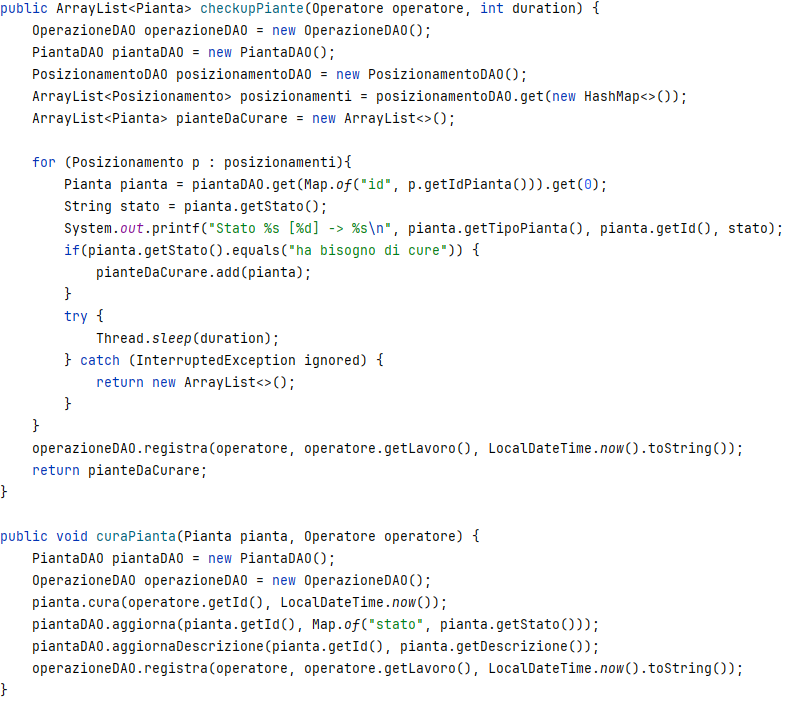
\includegraphics[scale=0.5]{resources/images/Snippets/snippet_checkuppiante_curapianta.png}
    \captionsetup{labelformat=empty, labelsep=none}
    \caption{Snippet 1: metodi \code{checkupPiante()} e \code{curaPianta()} nella classe \code{OperatoreController}}
    \label{fig:snippet_checkuppiante_curapianta}
\end{figure}

\subsubsection{AdminController}
In questa classe è presente il metodo \hyperref[fig:snippet_monitorasettore]{\code{monitoraSettore}} chiamato quando viene avviato un monitoraggio da parte dell'Admin. Se richiesto è lanciato anche \code{monitoraPosizioniBySettoreId} che fornisce dati su sensori e attuatori relativi alle Posizioni del Settore desiderato.\\
Anche qui sono presenti getters utili alla visualizzazione dei dati.

\begin{figure}[H]
    \centering
    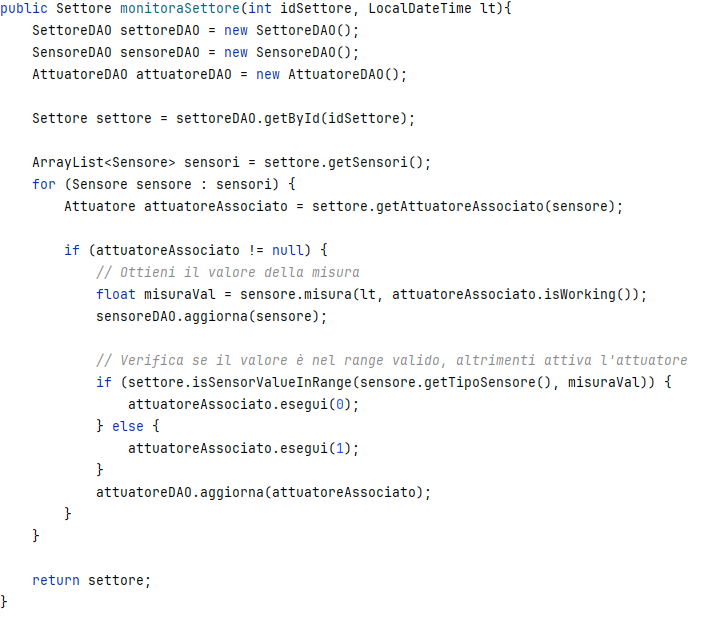
\includegraphics[scale=0.5]{resources/images/Snippets/snippet_monitorasettore.png}
    \captionsetup{labelformat=empty, labelsep=none}
    \caption{Snippet 2: metodo \code{monitoraSettore()} nella classe \code{AdminController}}
    \label{fig:snippet_monitorasettore}
\end{figure}

\subsubsection{AdminExtraController}
Infine con i metodi di AdminExtraController l’admin può fare il reset del database con \hyperref[fig:snippet_resetdatabase]{resetDatabase()} e inserire dei dati "default" con defaultDatabase(). Per la comunicazione con il database è utilizzata la classe AdminDAO.

\begin{figure}[H]
    \centering
    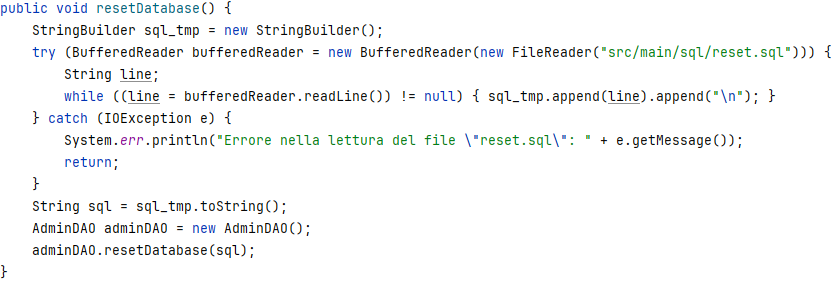
\includegraphics[scale=0.5]{resources/images/Snippets/snippet_resetdatabase.png}
    \captionsetup{labelformat=empty, labelsep=none}
    \caption{Snippet 3: metodo \code{resetDatabase()} nella classe \code{AdminExtraController}}
    \label{fig:snippet_resetdatabase}
\end{figure}

\subsection{ORM (Object-Relational Mapping)}
Nel package \code{main.java.ORM} (percorso \code{src/main/java/ORM}) sono implementate le interfacce per la comunicazione del sistema con un database. Per una gestione più coerente dei dati.\
Le classi "DAO" che appartengono a questo package si occupano di formulare e lanciare QUERY, eseguite tramite JDBC.

\subsubsection{ConnectionManager}
La classe si occupa di gestire la connessione al database per tutte le classi DAO tramite il metodo \hyperref[fig:snippet_connection_manager]{\code{getConnection()}}.
Essendo implementata seguendo il design pattern del \textit{Singleton} non è possibile che due DAO si colleghino contemporaneamente al database e quindi che si verifichino perdite di dati.\\
Inoltre questa classe contiene le informazioni esatte su l'URL, username e password per stabilire la connessione.

\begin{figure}[H]
    \centering
    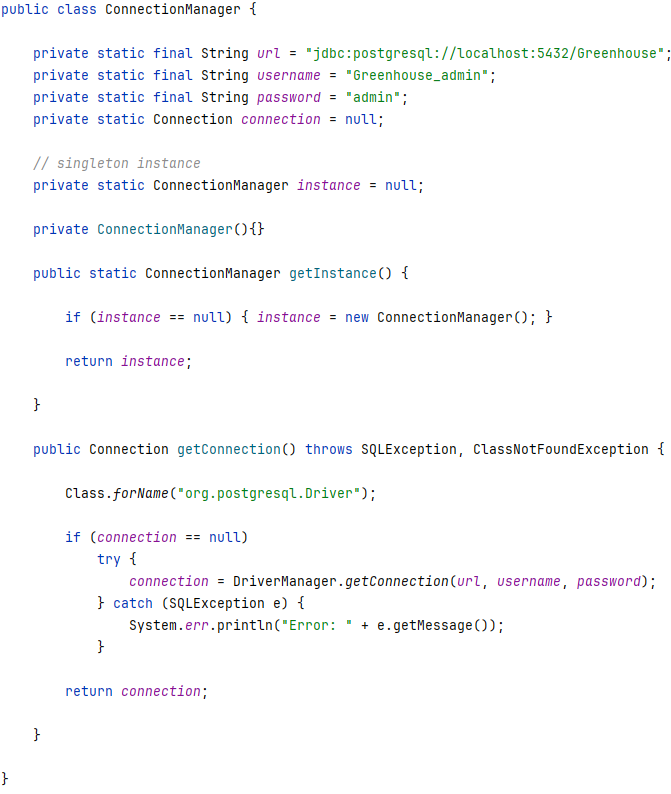
\includegraphics[scale=0.5]{resources/images/Snippets/snippet_connection_manager.png}
    \captionsetup{labelformat=empty, labelsep=none}
    \caption{Snippet 4: metodi \code{getInstance} e \code{getConnection()} nella classe \code{ConnectionManager}}
    \label{fig:snippet_connection_manager}
\end{figure}

\subsubsection{ClienteDAO}
La classe è preposta all'accesso al sistema tramite la funzione \hyperref[fig:snippet_clienteDAO]{\code{accedi(email, password)}} e alla registrazione (\hyperref[fig:snippet_clienteDAO]{\code{registra(...)}}) di un nuovo cliente. In più sono presenti i metodi per la modifica delle informazioni (\code{modificaAttributo(id\_cliente, ...)}) e per restituire un cliente presente in database in base a criteri specificati (\code{get(criteri)}).

\begin{figure}[H]
    \centering
    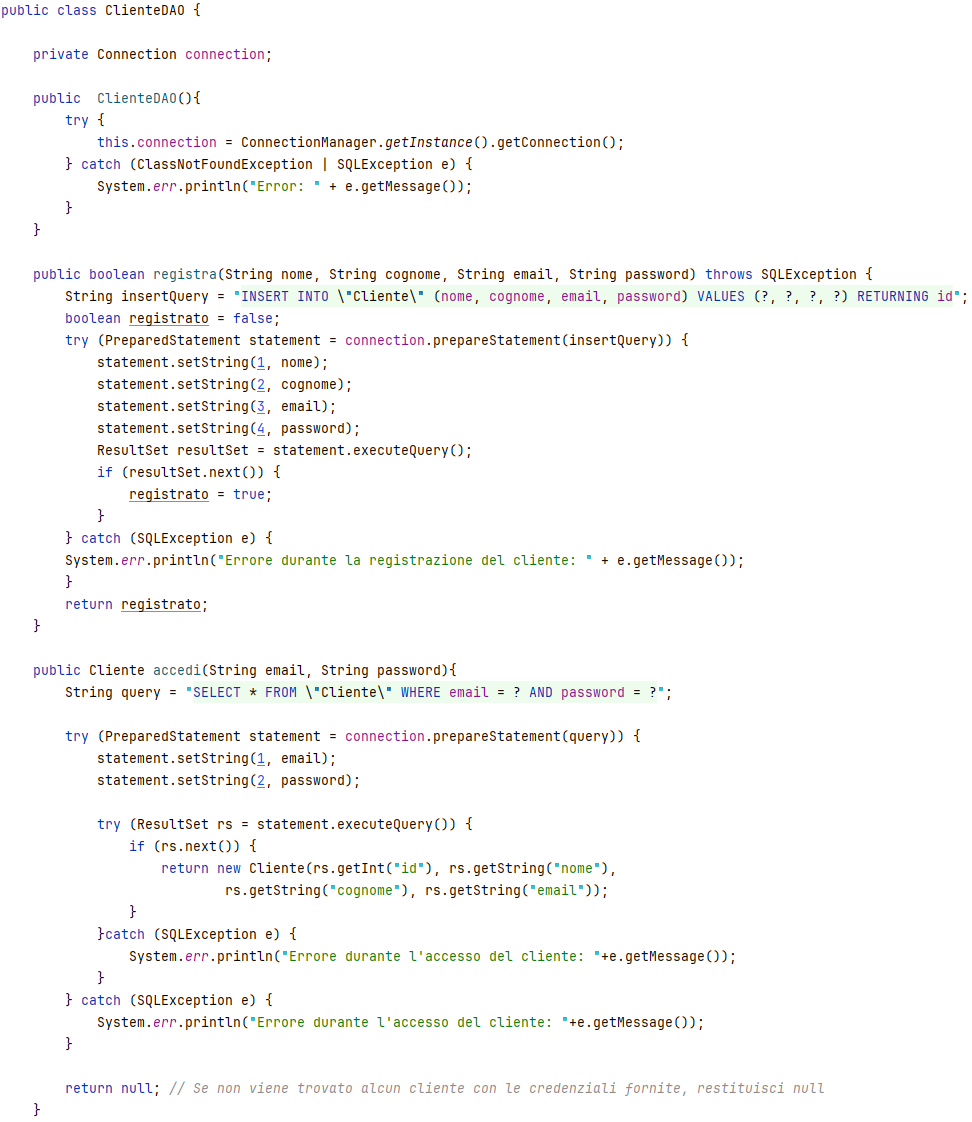
\includegraphics[scale=0.5]{resources/images/Snippets/snippet_clienteDAO.png}
    \captionsetup{labelformat=empty,labelsep=none}
    \caption{Snippet 5: metodi \code{registra()} e \code{accedi()} nella classe \code{ClienteDAO}}
    \label{fig:snippet_clienteDAO}
\end{figure}

\subsubsection{AdminDAO}
La classe svolge la funzione di accesso per l'admin come per il cliente ma ha anche i metodi   \\ \code{resetDatabase(sql), createDatabase(ql)} e \code{generateDefaultDatabase(sql)} che eseguono il reset.sql, schema.sql e defaul.sql tali da pulire e resettare il database.

\subsubsection{OperatoreDAO}
\code{OperatoreDAO} permette anch'esso l'accesso al sistema con funzione \code{accedi(email,password} con valore di ritorno un booleano. Ha anche un metodo \code{getById(id)} per restituire l'operatore a partire dall'Id richiesto.

\subsubsection{SensoreDAO, AttuatoreDAO e OperazioneDAO}
Le classi \code{SensoreDAO} e \code{AttuatoreDAO} restituiscono i rispettivi oggetti tramtie \code{getById(id)} e hanno anche il metodo \hyperref[fig:snippet_sensoreDAOaggiorna]{\code{aggiorna(sensore)}} (e \code{aggiorna(attuatore)}) utilizzato per aggiornare i parametri delle tabelle. La classe \code{OperazioneDAO} permette di tenere un record delle azioni degli attuatori tramite la funzione \code{registra(attuatore, descrizione, data)}.

\begin{figure}[H]
    \centering
    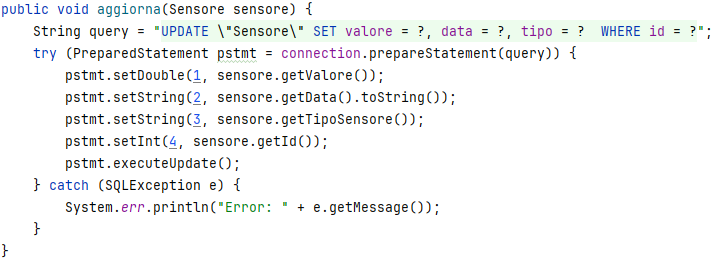
\includegraphics[scale=0.5]{resources/images/Snippets/snippet_sensoreDAOaggiorna.png}
    \captionsetup{labelformat=empty,labelsep=none}
    \caption{Snippet 6: metodo \code{aggiorna()} nella classe \code{SensoreDAO}}
    \label{fig:snippet_sensoreDAOaggiorna}
\end{figure}

\subsubsection{SettoreDAO, PosizioneDAO}
Mentre \code{SettoreDAO} ha solo due metodi per la creazione del settore (\code{getById(id)} e\code{get(criteri)}), \code{PosizioneDAO} non sono ha questi metodi ma anche metodi per assegnare , aggiornare e verificare se ci sono posizioni non assegnate.

\subsubsection{OrdineDAO e PiantaDAO}
\code{OrdineDAO} e \code{PiantaDAO}, come le altre DAO, hanno i metodi per inserire, aggiornare e restituire gli oggetti associati, inoltre \code{PiantaDAO} ha metodi per eliminare elementi, usato quando l'ordine è espletato.

\begin{figure}[H]
    \centering
    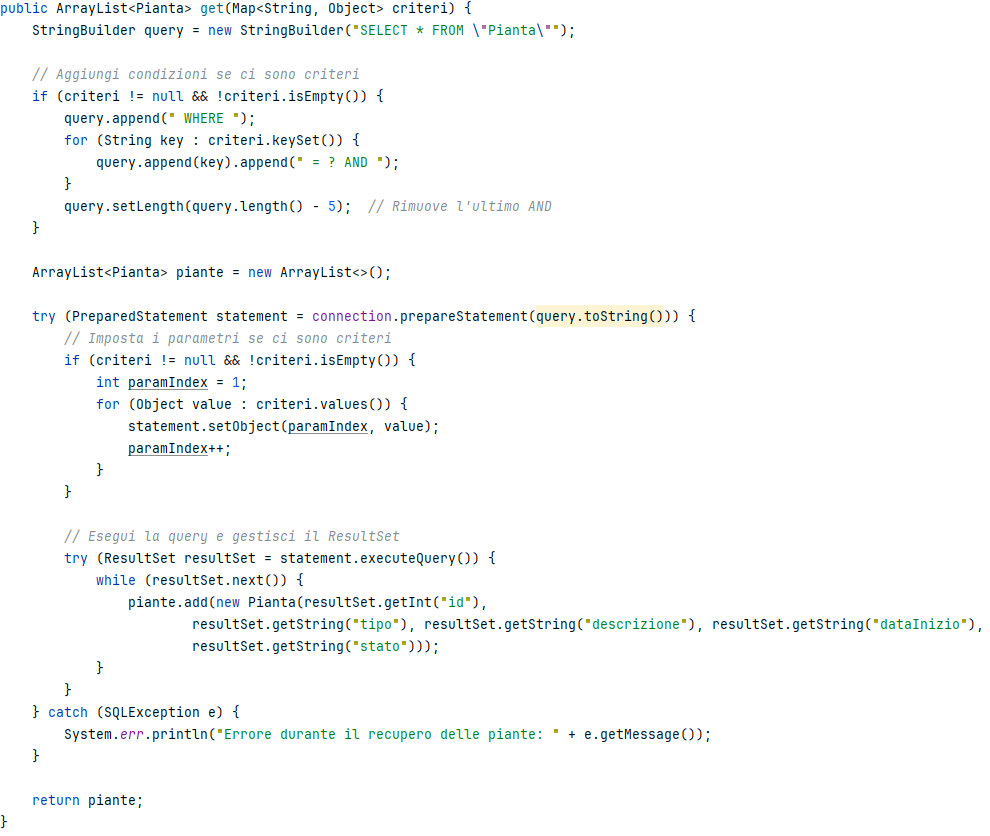
\includegraphics[scale=0.5]{resources/images/Snippets/snippet_piantaDAOget.png}
    \captionsetup{labelformat=empty,labelsep=none}
    \caption{Snippet 7: metodo \code{get()} nella classe \code{PiantaDAO}}
    \label{fig:snippet_piantaDAOget}
\end{figure}

\newpage

\subsubsection{PosizionamentoDAO}
La classe \code{PosizionamentoDAO} permette di ottenere i Posizionamenti richiesti dal database, aggiungerne di nuovi o eliminarli in base all'id dell'ordine di cui fanno parte (\hyperref[fig:snippet_eliminaposizionamentibyordine]{\code{snippet\_eliminaposizionamentibyordine()}}).

\begin{figure}[H]
    \centering
    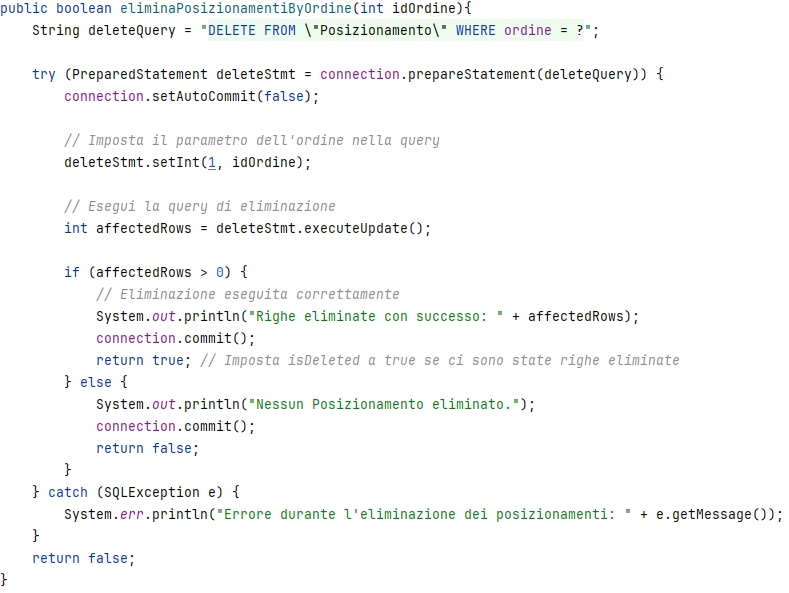
\includegraphics[scale=0.5]{resources/images/Snippets/snippet_eliminaposizionamentibyordine.png}
    \captionsetup{labelformat=empty,labelsep=none}
    \caption{Snippet 8: metodo \code{eliminaPosizionamentiByOrdine} della classe \code{PosizionamentoDAO}}
    \label{fig:snippet_eliminaposizionamentibyordine}
\end{figure}


\subsection{Database}
Per mantenere coerenza tra i dati del sistema è stato utilizzato un database utilizzando PostgreSQL, con il quale è possibile interfacciarsi tramite le classi DAO. Tale database segue lo schema delle operazioni CRUD (CREATE, READ, UPDATE, DELETE). \\
Per inizializzare il database sono stati creati 3 file \code{.sql}:
\begin{itemize}
    \item \code{reset.sql}: elimina tutte le tabelle del database (\code{DROP TABLE});
    \item \hyperref[fig:snippet_createtable]{\code{schema.sql}}: crea le tabelle del database definendo i vari attributi, chiavi e vincoli (\code{CREATE TABLE});
    \item \code{default.sql}: inserisce valori nelle tabelle in modo da avere uno stato iniziale già compatibile con il programma (\code{INSERT INTO}).
\end{itemize}
Questi 3 file sono stati eseguiti, grazie ai metodi presenti in AdminController, in fase di debug del programma e sono utilizzati anche prima di ogni test (\code{BeforeEach}) per impostare condizioni ben precise richieste dai test.

\begin{figure}[H]
    \centering
    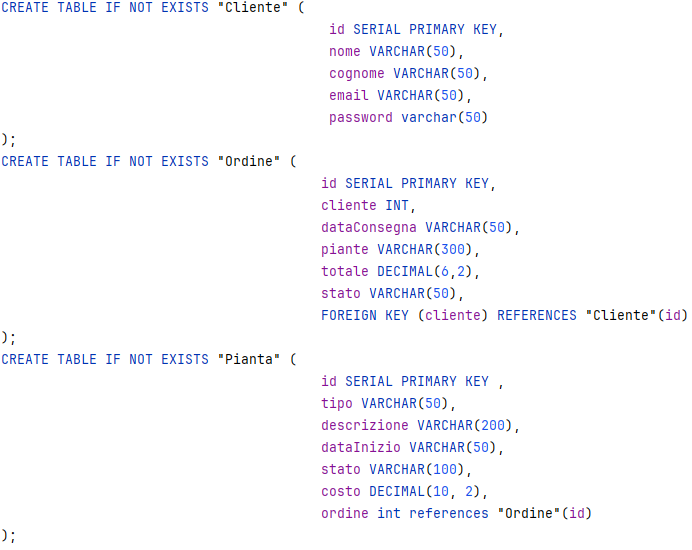
\includegraphics[scale=0.5]{resources/images/Snippets/snippet_createtable.png}
    \captionsetup{labelformat=empty,labelsep=none}
    \caption{Snippet 9: creazione tabelle \code{Cliente}, \code{Ordine} e \code{Pianta} nel file \code{schema.sql}}
    \label{fig:snippet_createtable}
\end{figure}


\subsection{Interfaccia}
Ai fini di debug e test del programma è stata implementata un'interfaccia da terminale che permette di fare il login ed eseguire azioni/compiti sul sistema.\\
È possibile navigare tra i menu inserendo da tastiera il numero corrispondente all'opzione scelta.\\
Laddove è richiesto, l'utente deve fornire certe stringhe in input (ad esempio le credenziali di accesso per il login).\\
Il diagramma dei menu disponibili si trova nella sezione \ref{subsec:nav-diagram}.

\begin{figure}[H]
    \centering
    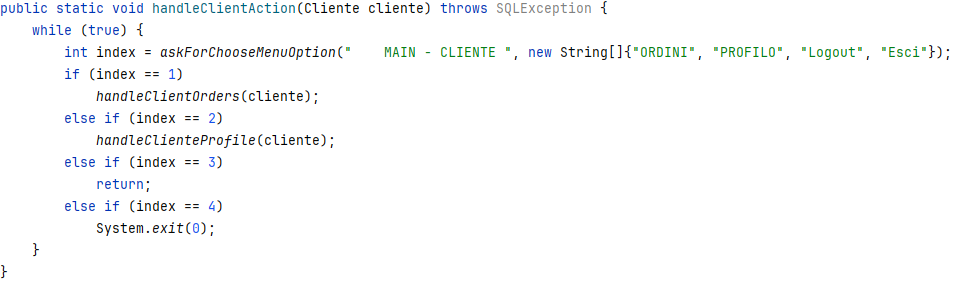
\includegraphics[scale=0.5]{resources/images/Snippets/snippet_handleclienteaction.png}
    \captionsetup{labelformat=empty,labelsep=none}
    \caption{Snippet 10: metodo \code{handleClienteAction} che mostra il menu principale del \code{Cliente}}
    \label{fig:snippet_handleclienteaction}
\end{figure}

\begin{figure}[H]
    \centering
    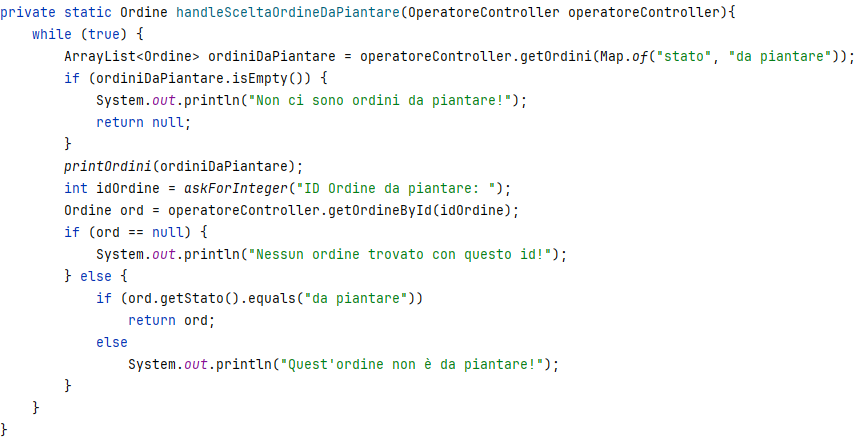
\includegraphics[scale=0.5]{resources/images/Snippets/snippet_handlesceltaordinedapiantare.png}
    \captionsetup{labelformat=empty,labelsep=none}
    \caption{Snippet 11: metodo \code{handleSceltaOrdineDaPiantare}}
    \label{fig:snippet_handlesceltaordinedapiantare}
\end{figure}


\section{Testing}
Per verificare la correttezza e funzionalità del programma sono stati realizzati dei test (vedi cartella \code{test} in \code{/src}). Questi riguardano quelle funzioni associate agli use cases obiettivo del progetto, quindi principalmente la BusinessLogic, che è la parte più "ad alto livello" del programma e che contiene le funzioni direttamente chiamate dall'interfaccia. \\
È presente anche un test per il DomainModel.\\
La sezione di ORM non presenta test in quanto si occupa "soltanto" di comunicare con il Database.

\subsection{Business Logic Test}
Molti di questi test presentano più variazioni, in quanto verificano sia il caso in cui le condizioni per una certa funzione siano favorevoli, quindi è atteso un esito positivo ("Success"), sia il caso in cui vengano riscontrati problemi e quindi ci si aspetta un esito negativo ("Fail").\\
I test sono suddivisi in più classi (rispettando la suddivisione che hanno le relative funzioni): \\
\code{LoginClienteControllerTest}, \code{LoginPersonaleControllerTest}, \code{ClienteControllerTest}, \code{OperatoreControllerTest}.

\subsubsection{LoginClienteControllerTest}
\begin{itemize}
    \item \code{setUp}: reimposta il database a uno stato iniziale default;
    \item \code{registrationTest\_Success}: esegue il test del metodo \code{registrati} di \code{loginClienteController}, utilizzata per la registrazione di un nuovo cliente;
    \item \code{registrationTest\_Fail}: come \code{registrationTest\_Success}, ma l'\code{email} con il quale si tenta di registrarsi appartiene a un cliente già presente nel database, quindi il test di aspetta un fallimento nella procedura;
    \item \code{loginTest\_Success}: verifica la corretta funzionalità del metodo \code{accedi} che permette al cliente di accedere al sistema;
    \item \code{loginTest\_Fail1} e \code{loginTest\_Fail2}: verifica l'effettivo fallimento del login nel caso in cui la \code{password} o l'\code{email} non siano corrette;    
\end{itemize}

\begin{figure}[H]
    \centering
    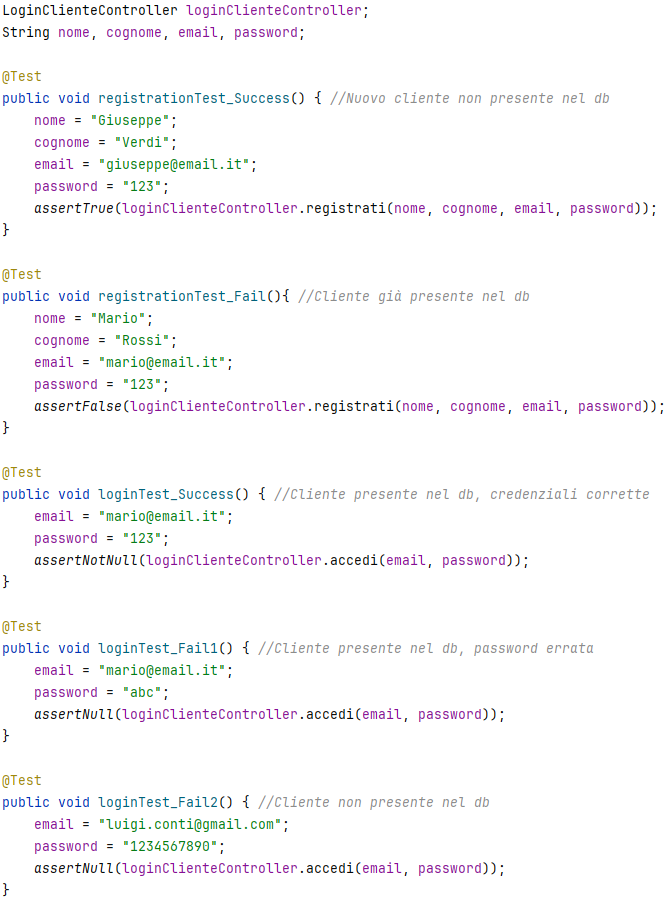
\includegraphics[scale=0.5]{resources/images/Snippets/snippet_LoginClienteControllerTest.png}
    \captionsetup{labelformat=empty,labelsep=none}
    \caption{Snippet 12: test di \code{LoginClienteControllerTest}}
    \label{fig:snippet_LoginClienteControllerTest}
\end{figure}

\newpage

\subsubsection{LoginPersonaleControllerTest}
Analogo a \code{LoginClienteControllerTest}, effettua i test di accesso nel sistema, ma da parte del personale lavorativo (\code{Admin} e \code{Operatore}) e contiene i seguenti test: \code{registrationTest\_Fail}, \code{loginAdmin\_Fail1}, \code{loginAdmin\_Fail2}, \code{loginOperatore\_Success}, \code{loginOperatore\_Fail1} e \code{loginOperatore\_Fail2}.

\begin{figure}[H]
    \centering
    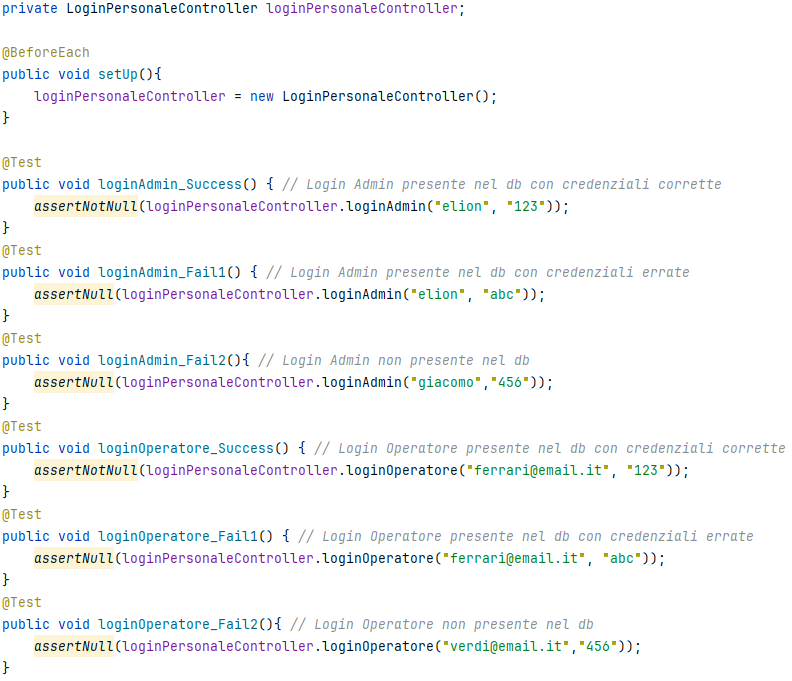
\includegraphics[scale=0.5]{resources/images/Snippets/snippet_LoginPersonaleControllerTest.png}
    \captionsetup{labelformat=empty,labelsep=none}
    \caption{Snippet 13: test di \code{LoginPersonaleControllerTest}}
    \label{fig:snippet_LoginPersonaleControllerTest}
\end{figure}

\subsubsection{ClienteControllerTest}
Verifica il corretto funzionamento dei metodi di \code{ClienteController}, quindi delle funzionalità a disposizione dei Clienti. Sono testate le funzioni di aggiornamento dei dati del profilo, richiesta nuovo ordine (Success e Fail), pagamento e ritiro di un ordine (Success e Fail);
\begin{itemize}
    \item \code{testAggiornaProfilo}: chiama il metodo \code{aggiornaProfilo} di \code{ClienteController}, e modifica il \code{nome} del cliente;
    \item \code{testRichiediNuovoOrdine\_Success}: crea un nuovo ordine e invia la richiesta al sistema. Si aspetta che tale ordine sia accettato senza problemi;
    \item \code{testRichiediNuovoOrdine\_Fail}: come il precedente, ma il numero di piante richiesto è superiore alla capacità dell'impianto, quindi la richiesta fallisce;
    \item \code{testPagaERitiraOrdine}: verifica che il metodo \code{pagaERitiraOrdine} di \code{ClienteController} funzioni correttamente.
\end{itemize}

\begin{figure}[H]
    \centering
    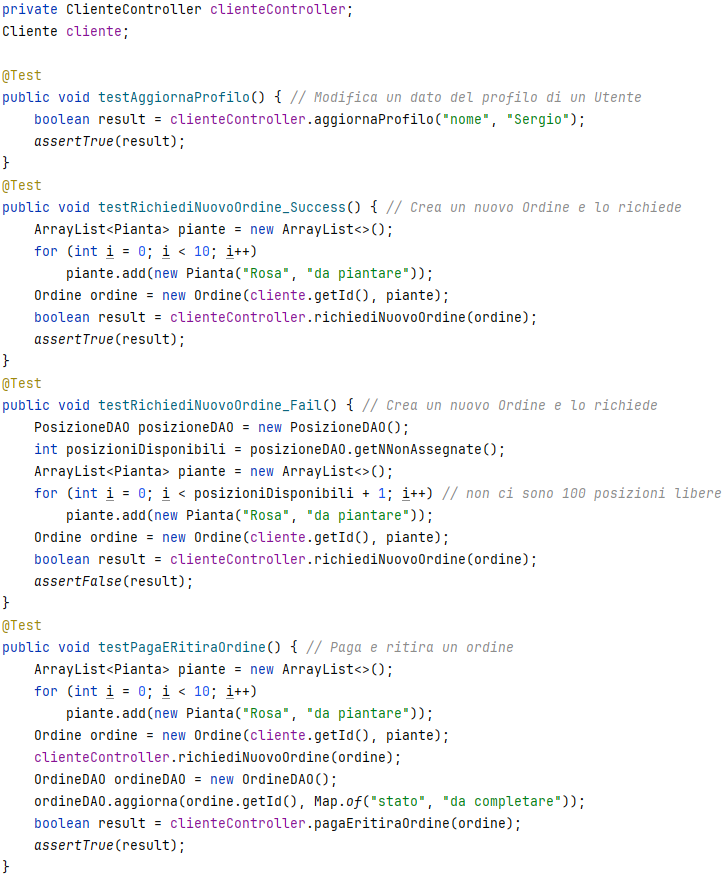
\includegraphics[scale=0.5]{resources/images/Snippets/snippet_ClienteControllerTest.png}
    \captionsetup{labelformat=empty,labelsep=none}
    \caption{Snippet 14: test di \code{ClienteControllerTest}}
    \label{fig:snippet_ClienteControllerTest}
\end{figure}

\subsubsection{OperatoreControllerTest}
\begin{itemize}
    \item \code{completaOrdineTest\_Success}: verifica che il completamento di un ordine venga eseguito correttamente;
    \item \code{completaOrdineTest\_Fail}: prova ad eseguire il completamento di un ordine che non è ancora stato piantato, perciò si aspetta un fallimento;
    \item \code{checkupPianteTest\_Success}: test del check-up delle piante eseguito da parte di un operatore. Alcune piante vengono (forzatamente) impostate come bisognose di cure e si verifica che queste vengano tutte rilevate durante il check-up;
    \item \code{checkupPianteTest\_Fail}: nessuna pianta ha bisogno di cure (in base a questo setup), quindi il check-up non rileva piante bisognose;
    \item \code{curaPiantaTest}: chiama il metodo \code{curaPianta} di \code{OperatoreController} e ne verifica il funzionamento;
    \item \code{piantaOrdineTest}: testa la funzione utilizzata per piantare un ordine.
\end{itemize}

\begin{figure}[H]
    \centering
    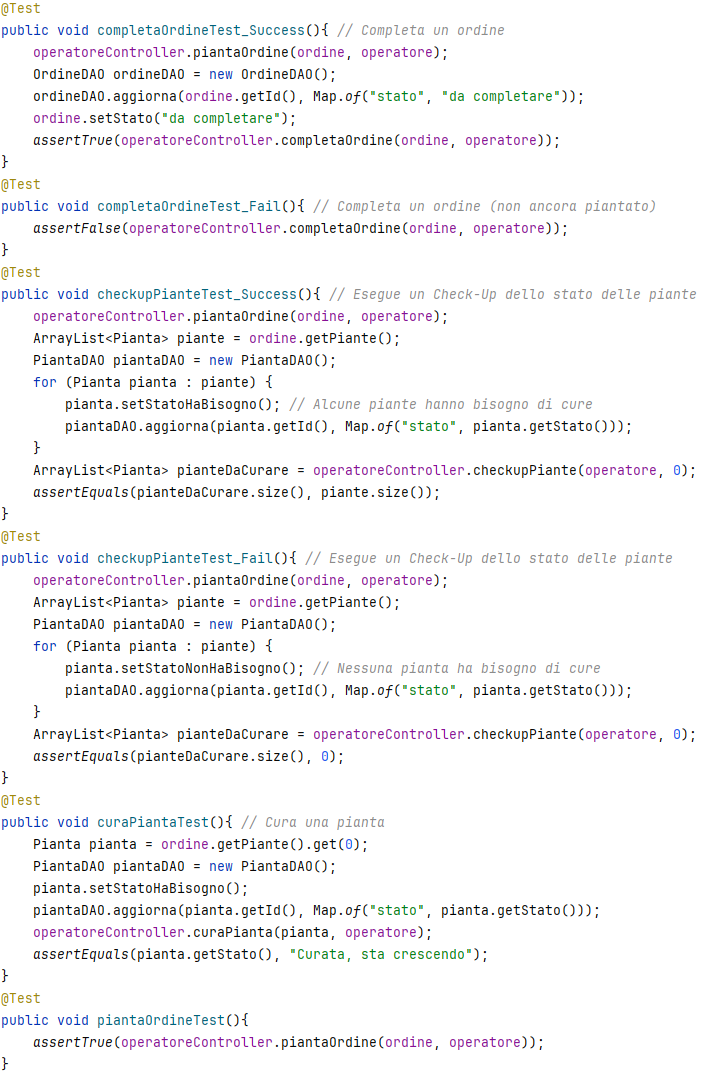
\includegraphics[scale=0.65]{resources/images/Snippets/snippet_OperatoreControllerTest.png}
    \captionsetup{labelformat=empty,labelsep=none}
    \caption{Snippet 15: test di \code{OperatoreControllerTest}}
    \label{fig:snippet_OperatoreControllerTest}
\end{figure}

\subsection{Domain Model Test}
Per quanto riguarda il Domain Model è stato effettuato un solo test, in quanto sono presenti classi che fungono soltanto da entità, e generalmente sono passive, cioè prive di metodi e funzionalità.\\
I sensori però contengono un metodo \code{misura} che prende in ingresso l'orario e lo stato dell'attuatore associato a tale sensore e ritorna una misurazione del parametro fisico che gli compete. Questo simula l'influenza del tempo e degli attuatori sulla misurazione.\\
Nel caso in cui l'\code{Irrigatore} sia acceso (\hyperref[fig:snippet_IgrometroTerraTest]{\code{testMisura\_Irr\_ON}}), ci si aspetta un valore di umidità del terreno (misurato da \code{IgrometroTerra}) crescente nel tempo. Altrimenti (\hyperref[fig:snippet_IgrometroTerraTest]{\code{testMisura\_Irr\_OFF}}) il valore diminuisce (l'acqua viene assorbita dalla pianta). Il test verifica questo.

\begin{figure}[H]
    \centering
    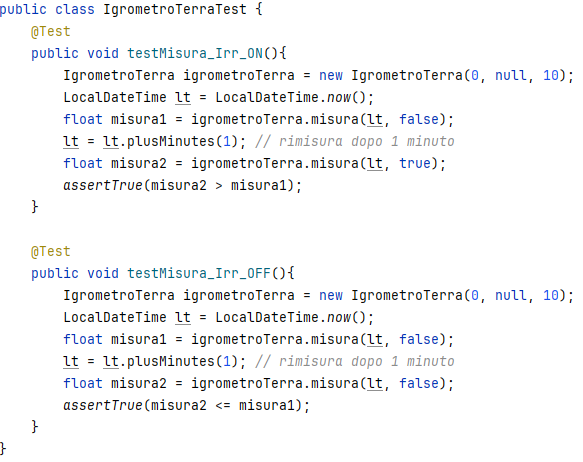
\includegraphics[scale=0.5]{resources/images/Snippets/snippet_IgrometroTerraTest.png}
    \captionsetup{labelformat=empty,labelsep=none}
    \caption{Snippet 16: test di \code{IgrometroTerra}}
    \label{fig:snippet_IgrometroTerraTest}
\end{figure}

\end{document}
